%% Version 4.3.2, 25 August 2014
%
%%%%%%%%%%%%%%%%%%%%%%%%%%%%%%%%%%%%%%%%%%%%%%%%%%%%%%%%%%%%%%%%%%%%%%
% Template.tex --  LaTeX-based template for submissions to the 
% American Meteorological Society
%
% Template developed by Amy Hendrickson, 2013, TeXnology Inc., 
% amyh@texnology.com, http://www.texnology.com
% following earlier work by Brian Papa, American Meteorological Society
%
% Email questions to latex@ametsoc.org.
%
%%%%%%%%%%%%%%%%%%%%%%%%%%%%%%%%%%%%%%%%%%%%%%%%%%%%%%%%%%%%%%%%%%%%%
% PREAMBLE
%%%%%%%%%%%%%%%%%%%%%%%%%%%%%%%%%%%%%%%%%%%%%%%%%%%%%%%%%%%%%%%%%%%%%

%% Start with one of the following:
% DOUBLE-SPACED VERSION FOR SUBMISSION TO THE AMS
\documentclass{ametsoc}


% TWO-COLUMN JOURNAL PAGE LAYOUT---FOR AUTHOR USE ONLY
%\documentclass[twocol]{ametsoc}

\usepackage{multirow}
\usepackage{gensymb}
\usepackage{subcaption}
\usepackage{xcolor,colortbl}

% After http://tex.stackexchange.com/questions/94799/how-do-i-color-table-columns-and-rows
\newcommand{\mc}[2]{\multicolumn{#1}{c}{#2}}
\definecolor{Gray}{gray}{0.85}
\definecolor{LightCyan}{rgb}{0.88,1,1}
\newcolumntype{a}{>{\columncolor{Gray}}c}

%%%%%%%%%%%%%%%%%%%%%%%%%%%%%%%%
%%% To be entered only if twocol option is used

\journal{jcli}

%  Please choose a journal abbreviation to use above from the following list:
% 
%   jamc     (Journal of Applied Meteorology and Climatology)
%   jtech     (Journal of Atmospheric and Oceanic Technology)
%   jhm      (Journal of Hydrometeorology)
%   jpo     (Journal of Physical Oceanography)
%   jas      (Journal of Atmospheric Sciences)	
%   jcli      (Journal of Climate)
%   mwr      (Monthly Weather Review)
%   wcas      (Weather, Climate, and Society)
%   waf       (Weather and Forecasting)
%   bams (Bulletin of the American Meteorological Society)
%   ei    (Earth Interactions)

%%%%%%%%%%%%%%%%%%%%%%%%%%%%%%%%
%Citations should be of the form ``author year''  not ``author, year''
\bibpunct{(}{)}{;}{a}{}{,}

%%%%%%%%%%%%%%%%%%%%%%%%%%%%%%%%

%%% To be entered by author:

%% May use \\ to break lines in title:

\title{Global Optimization of the Analogue Method by Means of Genetic Algorithms}

%%% Enter authors' names, as you see in this example:
%%% Use \correspondingauthor{} and \thanks{Current Affiliation:...}
%%% immediately following the appropriate author.
%%%
%%% Note that the \correspondingauthor{} command is NECESSARY.
%%% The \thanks{} commands are OPTIONAL.

    %\authors{Author One\correspondingauthor{Author One, 
    % American Meteorological Society, 
    % 45 Beacon St., Boston, MA 02108.}
% and Author Two\thanks{Current affiliation: American Meteorological Society, 
    % 45 Beacon St., Boston, MA 02108.}}

\authors{Pascal Horton\correspondingauthor{Terranum, Rue de l'industrie 35 bis, 1030 Bussigny, Switzerland.}}

%% Follow this form:
    % \affiliation{American Meteorological Society, 
    % Boston, Massachusetts.}

\affiliation{University of Lausanne and Terranum, Lausanne, Switzerland}

%% Follow this form:
    %\email{latex@ametsoc.org}

\email{pascal.horton@alumnil.unil.ch}

%% If appropriate, add additional authors, different affiliations:
    %\extraauthor{Extra Author}
    %\extraaffil{Affiliation, City, State/Province, Country}

\extraauthor{Michel Jaboyedoff}
\extraaffil{University of Lausanne, Lausanne, Switzerland}

%% May repeat for a additional authors/affiliations:

%\extraauthor{}
%\extraaffil{}

\extraauthor{Charles Obled}
\extraaffil{Universit\'{e} de Grenoble-Alpes, LTHE, Grenoble, France}

%%%%%%%%%%%%%%%%%%%%%%%%%%%%%%%%%%%%%%%%%%%%%%%%%%%%%%%%%%%%%%%%%%%%%
% ABSTRACT
%
% Enter your abstract here
% Abstracts should not exceed 250 words in length!
%
% For BAMS authors only: If your article requires a Capsule Summary, please place the capsule text at the end of your abstract
% and identify it as the capsule. Example: This is the end of the abstract. (Capsule Summary) This is the capsule summary. 

\abstract{The analogues method is based on a statistical relationship between synoptic atmospheric variables and local weather, which we aim at forecasting. This relationship is expressed through many parameters that are usually calibrated by means of a semi-automatic procedure. This classic calibration is relatively fast and provide acceptable results, but it has strong constraints, is made of successive steps and thus cannot handle parameters dependencies, and mainly, it cannot calibrate automatically some parameters, such as the selection of the pressure levels and the temporal windows on which the predictors are compared. In order to surpass these limitations, we assessed a global optimization technique, namely genetic algorithms, that can optimize jointly all parameters of the method and thus provide a global optimum by taking into account the parameters dependencies. Moreover, it can calibrate parameters that were previously manually assessed, and can take into account new degrees of freedom that were unthinkable before. 
These kind of optimization techniques need however to be tailored to the problem to solve. We had to assess multiple combinations of algorithms, and even to develop new operators, such as the \textit{chromosome of adaptive search radius} which was found to be very robust, in order to make recommendations for the use of genetic algorithms to optimize the analogue method. These recommendations are the primary outcome of this work, as it opens new perspective for the improvement of the analogue method, and its application to new regions or to new predictands.
We then applied the optimizer to the Rh\^{o}e catchment in the Swiss Alps and obtained coherent results which significantly improve the performance of the forecasting by analogy. The optimizer allowed us to calibrate jointly all parameters of the method and to add a weighting of the criteria per pressure level, as well as non-overlapping spatial windows.}

\begin{document}

%% Necessary!
\maketitle


%%%%%%%%%%%%%%%%%%%%%%%%%%%%%%%%%%%%%%%%%%%%%%%%%%%%%%%%%%%%%%%%%%%%%
% MAIN BODY OF PAPER
%%%%%%%%%%%%%%%%%%%%%%%%%%%%%%%%%%%%%%%%%%%%%%%%%%%%%%%%%%%%%%%%%%%%%
%

%% In all cases, if there is only one entry of this type within
%% the higher level heading, use the star form: 
%%
% \section{Section title}
% \subsection*{subsection}
% text...
% \section{Section title}

%vs

% \section{Section title}
% \subsection{subsection one}
% text...
% \subsection{subsection two}
% \section{Section title}

%%%
% \section{First primary heading}

% \subsection{First secondary heading}

% \subsubsection{First tertiary heading}

% \paragraph{First quaternary heading}


\section{Introduction}
\label{section_intro}

The analogue method is a downscaling technique based on the idea expressed by \citet{Lorenz1969}, that similar situations in terms of atmospheric circulation are likely to lead to similar local weather \citep{Bontron2005}. It aims at forecasting a predictand, often the daily precipitation, on the basis of predictor variables describing the synoptic atmospheric circulation. Many parameters define this relationship, which are usually calibrated by means of a semi-automatic procedure.


\subsection{The analogue method}
\label{section_analog_method}

Multiple variations of the methods exist, and some aspects and parameters will not be detailed hereafter. There are mainly 2 parametrizations that are used most often: one that relies on an analogy of the atmospheric circulation, and another that adds a second level of analogy on humidity variables \citep{Obled2002, Bontron2005, Marty2012}.

The method based on the analogy of the synoptic circulation consists in the following steps (Table \ref{table:params_R1}): We assess the similarity of the atmospheric circulation of a target date with every day of the archive by processing the S1 criteria \citep[Eq.\ (\ref{eq:S1}), ][]{Teweles1954, Drosdowsky2003}, which is a comparison of gradients, over a certain spatial window. \citet{Bontron2005} showed that the geopotential height at 500~hPa and 1000~hPa are the best first predictors of the NCEP/NCAR reanalysis dataset, and that the S1 criteria performs better than scores based on absolute distances. The reason for such better results is that the S1 criteria allows comparing the circulation pattern, by means of the gradients, rather than the absolute value of the geopotential height. To cope with seasonal effects, candidate dates are extracted within a period of 4 months centred around the target date, for every year of the archive.

\begin{equation}
\label{eq:S1}
S1=100 \frac {\displaystyle \sum_{i} \vert \Delta\hat{z}_{i} - \Delta z_{i} \vert}
{\displaystyle \sum_{i} max\left\lbrace \vert \Delta\hat{z}_{i} \vert , \vert \Delta z_{i} \vert \right\rbrace }
\end{equation}
where $\Delta \hat{z}_{i}$ is the forecast geopotential height difference between the \textit{i}th pair of adjacent points in the target situation, and $\Delta z_{i}$ is the corresponding observed geopotential height difference in the candidate situation. The differences are processed separately in both directions. The smaller the S1 values are, the more similar the pressure fields.

The $N_{1}$ dates with the lowest values of S1 are considered as analogues to the target day. The number of analogues, $N_{1}$, is a parameter to calibrate. Then, the daily observed precipitation amount of the $N_{1}$ resulting dates provide the empirical conditional distribution considered as the probabilistic forecast for the target day.

The other most know parametrization adds a second level of analogy on humidity variables (Table \ref{table:params_R2}). The predictor that \citet{Bontron2004} found optimal for the France territory is a humidity index made of the product of the precipitable water with the relative humidity at 850~hPa. \cite{Horton2012a} confirmed that this index is better for the Swiss Alps than any other variable from the NCEP/NCAR reanalysis considered independently. When adding a second level of analogy, we subsample $N_{2}$ dates in the $N_{1}$ analogues on the atmospheric circulation, to end up with a smaller number of analogue situations. When we add a second level of analogy, we keep a higher number of analogues on the first level.


\subsection{Data}
\label{section_data}

The analogue method relies on two types of data: predictors, that are atmospheric variables describing the state of the atmosphere at a synoptic scale, and the predictand, which is the local weather time series we want to forecast.

Predictors are generally reanalysis datasets (and outputs of a global numerical weather prediction models for the target situation in operational forecasting, which is not the topic of this paper). We will work here with the NCEP/NCAR reanalysis \citep[6-hourly, 17 pressure levels at a resolution of 2.5\degree, see][]{Kalnay1996}, but it can be any other reanalysis dataset.

The predictand (which is to be predicted) is in our case the daily precipitation (6~a.m. to 6~a.m. the next day) measured at the MeteoSwiss' stations network, for the period 1961-2008. The time series from every available gauging station were averaged over subregions in order to smooth local effects \citep{Obled2002, Marty2012}.


\subsection{Calibration framework}

The calibration of the analogue method is usually carried out in a perfect prognosis \citep{Klein1959} framework \citep{BenDaoud2010, Bontron2004}. Perfect prognosis uses observed or reanalyzed data to calibrate the relationship between predictors and predictands. Then, when used in operational forecasting, this relationship is applied to global model forecasts, that contains larger uncertainties. This framework allow us to identify relationships that are as close as possible to the natural links between predictors and predictands, by reducing uncertainties related to numerical forecasting models. However, no model is perfect, and even reanalysis data contain a bias that cannot be ignored. For this reason, the statistical relationships identified in the perfect prognosis framework should be applied to model outputs that are as similar as possible to the model used to elaborate the reanalysis. 

Another reason for working in a perfect prognosis framework is that numerical models evolve continuously, and so does the forecast they provide. Re-forecasts would allow us to work on a homogeneous dataset, as they are regularly reprocessed. However, we would need to redo the calibration procedure every time a new version is available, in order to reduce the bias \citep{Wilson2002}. Moreover, the reforecasts are not re-processed for every new version of the model, meaning we still end up with a bias between the forecast and the archive. Finally, the length of reanalyses datasets are usually much longer than reforecast datasets, which allows us to identify more robust relationships. The size of the archive is indeed an important criteria for the analogue method.

The statistical relationship is established on a calibration period that is as long as possible. For every day of this period, a search for analogues is processed, the precipitation data are associated with the corresponding dates and a forecast score is calculated. During the search for analogues situations, 120 days around the target date are excluded (thus excluding data in the same year) in order to consider only truly independent candidates days.

A validation period is always considered. It consists of an independent period that is never used as target neither candidate date. Validating the parameters of the analogue method is very important in order to avoid over-parametrization and thus to ensure that the statistical relationship is valid on another period.

The accuracy of the parameters is evaluated by means of the CRPS \citep[Continuous Ranked Probability Score,][]{Brown1974, Matheson1976, Hersbach2000}. It allows assessing the predicted cumulative distribution functions $F(y)$ compared to the observed value $y^{0}$. The better the forecast, the smaller the score. The mean CRPS of a forecast series of length $n$ can be written:

\begin{equation}
\label{eq:CRPS}
CRPS = \frac{1}{n} \sum_{i=1}^{n} \left(  \int_{-\infty}^{+\infty} \left[ F_{i}(y)-H_{i}(y-y_{i}^{0})\right]^{2} dy \right) 
\end{equation}
where $H(y-y_{i}^{0})$ is the Heaviside function that is null when $y-y_{i}^{0}<0$, and has the value 1 otherwise. The mean CRPS is averaged on the calibration, respectively the validation periods, on all days, may they be dry, slightly rainy or with heavy precipitation.

This score is now commonly used for the evaluation of continuous variables prediction systems \citep{Casati2008, Marty2010}. To compare the value of the score in regard to a reference, we often consider its skill score value, and use the climatological distribution as the reference. The CRPSS (\textit{Continuous Ranked Probability Skill Score}) is thus defined as following:

\begin{equation}
\label{eq:CRPSS}
CRPSS = \dfrac{CRPS-CRPS_{r}}{CRPS_{p}-CRPS_{r}} = 1-\dfrac{CRPS}{CRPS_{r}}
\end{equation}
where $CRPS_{r}$ is the CRPS value for the reference and $CRPS_{p}$ would be the one for a perfect forecast ($CRPS_{p} = 0$).


\subsection{The classic calibration approach}

The calibration procedure that we call ''classic'' was developed by \citet{Bontron2004} at the LTHE laboratory (INPG, Grenoble). It determines the optimal parameters for the different variables of each level of analogy. The analogy levels (eg the atmospheric circulation or humidity index) are calibrated sequentially. The procedure consists of the following steps \citep{Bontron2004}:

\begin{enumerate}
	\item Manual selection of the following parameters:
	\begin{enumerate}
		\item meteorological variable,
		\item pressure level,
		\item temporal window (hour of observation),
		\item initial analogue numbers.
	\end{enumerate}
	
	\item For every level of analogy:
	\begin{enumerate}
		\item Identification of the most skilled unitary cell (1 point for humidity variables and 4 for the geopotential height when using the S1 criteria) over a large domain. Every point (or cell) of the full domain is assessed jointly on all predictors of the level of analogy (consisting generally of the same variable, but on different pressure levels and at different hours).
		\item From this most skilled point, the spatial window is expanded by successive iterations in the direction of greater performance gain. The detailed stages are the followings: (i) The unitary spatial window is expanded in every 4 directions successively. The performance score is processed for these 4 windows. (ii) Only the direction providing the best improvement is applied to our spatial window. (iii) From this new spatial window, an increase in every 4 directions is once again assessed, and the best improvement is applied. (iv) The spatial window grows up by repeating the previous steps, until no improvement is reached.
		\item The number of analogues is optimized for the current level of analogy.
		\item A new level of analogy can be added, based on other variables (such as the humidity index) on predefined pressure levels and time frames. The number of analogues for the next level of analogy is initiated at a chosen value. Then, the procedure starts again from step (a) for the new level. The parameters calibrated on the previous analogue levels are fixed and do not change (except the number of analogues, at the final stage). 
	\end{enumerate}
	\item Finally, the numbers of analogues are re-assessed for the different levels of analogy. This is done iteratively by varying the number of analogues of each level in a systematic way.
\end{enumerate}

The calibration is thus done in successive steps. Previously calibrated parameters are generally not reassessed. The advantage of this method is that it is fast, it provides acceptable results, and it has low computing requirements. We added small improvements to this method by allowing the spatial windows to do other moves, such as: (1) increase in 2 simultaneous directions, (2) decrease in 1 or 2 simultaneous directions, (3) expansion or contraction (in every direction), (4) shift of the window (without resizing) in 8 directions (including diagonals), and finally (5) all the moves described above, but with a factor of 2, 3, or more. For example, we try to increase by 2 units in one (or more) direction. This allows to skip one size that may not be optimal.

These supplementary steps often result in spatial windows that are a bit different, but the performance gain is rather marginal. These methods are available in the open source software AtmoSwing (Analogue Technique MOdel for Statistical Weather forecastING, www.atmoswing.org).


\subsection{Motivation for a global optimization}

The classic calibration is fast to optimize one spatial window for a given pressure level and temporal window. However, it doesn't provide an objective selection of the pressure level and temporal window. The only option is to try systematically every combination, which may be acceptable for no more than 2 levels. However, \citet{Horton2012a} showed that additional pressure levels may improve the method.

We observed during the calibration of the analogue method that the resulting parameters vary with the initial choices (such as the number of analogues). In addition, the different levels of analogy (eg on the atmospheric circulation and the humidity index) are always calibrated sequentially. However, we can not exclude any dependency between them, which could lead us to select another parametrization if we calibrate them together. Simultaneous calibration of all parameters has never been undertaken so far. Only a global optimization technique can be able to optimize all parameters of all analogy levels simultaneously.

When creating the classic calibration procedure, \citet{Bontron2004} was aware of the problem of dependencies between parameters and wrote: '' \textit{We perceive here the combinatorial aspect of our problem: variables and spatial windows are not independent. We will present our results by first searching the best variable [note: e.g. selection of the pressure level and the temporal window for the geopotential height] on a chosen spatial window, and next, the best window for the chosen variable. However, even by repeating the process, are we sure to obtain the optimal combination?} ''. And later in his work: '' \textit{Our approach, which is again to vary the parameters one by one -- the others being fixed in a more or less arbitrary manner -- may therefore not exactly lead us to the optimal solution} ''. \citet{Bliefernicht2010} has also faced the combinatorial issue of the parameters of the analogue method and concludes that one needs to be an expert to know their respective influence, their sensitivity and their nonlinear interactions. \citet{BenDaoud2010}, when calibrating the analogue method, also stated that '' \textit{the combinatory aspect related to the calibration was found to be too high for all the parameters to be calibrated simultaneously } ''.

The analogue method needs to be adapted to every new region it is applied, because the leading meteorological influences are specific to this region. Even the selection of the pressure level and the temporal window should be reconsidered, when not the variable itself. For example, \citet{BenDaoud2010} found the vertical velocity relevant for the great plains in France, when \citet{Horton2012a} found no interest in this variable in an Alpine environment, because in the Alps, the vertical motion is mainly controlled by orographic effects, and was thus already well related to the atmospheric circulation itself. So, when adapting the analogue method to a new region, we should assess systematically every combination of pressure levels, time and spatial windows, which is an intensive task. This procedure can be automatized by a global optimization technique.

Our ambition was then to assess the feasibility of an automatic optimization of the analogue method through various techniques. The objective was to find an approach to optimize all parameters simultaneously, and thus be able to identify the global optimum in the parameter space. In addition, it can overcome the systematic manual assessments of certain parameters such as the selection of the pressure levels and time windows. Finally, it can open new perspectives by allowing the addition of new degrees of freedom, such as a weighting of the criteria values between the pressure levels, and the consideration of non-overlapping spatial windows between the pressure levels.

\citet{Horton2012a} assessed the ability of the \citet{Nelder1965a} method based on a simplex approach. This technique didn't provide satisfying results and failed at identifying the global optimum. Indeed, the results didn't converge and many local optimums came out. The parameter space of the analogue method is very complex and not appropriate for a linear optimization technique. Genetic algorithms were found to be much more relevant for such application.


\section{Adjusting genetic algorithms}

Genetic algorithms (GAs) come from the world of stochastic optimization, more specifically from metaheuristic approaches. These are stochastic iterative algorithms that behave like search algorithms by exploiting the characteristics of a problem and are particularly suitable for complex parameter spaces.

Genetic algorithms are part of the family of evolutionary algorithms \citep{Back1993b, Schwefel1993}, which get inspiration from some mechanisms of biological evolution, such as reproduction, genetic mutations, chromosomal crossovers, and natural selection. GAs are the most used technique from evolutionary algorithms \citep{Back1993b}, and they are constantly improving \citep{Haupt2004}. However, with time, the different methods of evolutionary algorithms tend to be similar and share many commonalities \citep{Back1996b, Haupt2004}.

The method was originally developed by \citet{Holland1992b} and popularized by \citet{Goldberg1989}. Unlike a linear or local optimization, GAs seek the global optimum on a complex surface, theoretically without restriction, but with no guarantee to reach it.


\subsection{Basic concepts of the genetic algorithms}

GAs mimic the evolution of a population of individuals in a new environment, by applying rules based on natural processes, such as DNA mutation, chromosomes crossover, natural selection, etc. It simulates the fact that in a natural environment, the most suitable individuals tend to survive longer, to reproduce more easily, and so to influence coming generations by providing genes that provide some good performance in a certain domain. Generation after generation, the DNA mixes and the strong genes cumulate in some individuals \citep{Beasley1996a}. Globally, the fitness of the population to its environment increases, while retaining enough variety to not converge too quickly to a local optimum.

Applications of GAs are very diversified as they can handle many parameters of various types \citep{Joines1996a}, even with very complex cost surfaces \citep{Haupt2004}. GAs work remarkably well with intervariable dependences \citep{Haupt2004}. The objective function to optimize (often named fitness function in this context) can be of different types (mathematical function, experimental or numerical modeling). Only the resulting value is used for optimization. Indeed, these algorithms do not require any knowledge of the problem, which can be used as black-box, but they must be adapted in order to perform optimally.

By means of the reproduction operator and the natural selection, the GAs focus on the most promising regions of the parameter space \citep{Holland1992b}. Points (parameter sets) are densified in these areas because the strong genes of the best individuals propagate from generation to generation.

Two conditions guarantee in theory the convergence to the global optimum \citep{Zitzler2004a}: (1) Parameters mutations that can allow to explore the entire parameter space, thereby ensures that any value can be achieved with a non-zero probability. (2) A rule of elitism ensuring that an optimal solution cannot be lost or damaged.

Practically, GAs allow rapidly approaching satisfactory solutions, but they do not provide the optimum solution for sure \citep{Zitzler2004a}. It is indeed mainly a matter of time. When the optimizer gets closer to the global optimum, any new improvement takes more time to appear (see figure \ref{fig:evolution}), and the final adjustment of the parameters is very time consuming \citep{Back1993a}. For problems that require a significant amount of time in order to evaluate the objective function, as in our case, we have to limit the number of generations to get reasonable processing time. Thus, different acceptable solutions can result from one or more optimizations \citep{Holland1992b}. This is a strength and a weakness of GAs: they are very good at exploring complex parameter spaces in order to identify the most promising areas, but they will not necessarily find the best solution with the optimal values of all parameters \citep{Holland1992b}.


\subsection{Structure and operators}

The GAs optimize a population of individuals (parameter sets). Each individual contains a chromosome (parameters of the analogue method in our case). We call gene every parameter that constitutes the chromosome. The parameters to optimize have long been coded in binary form and assembled as strings in the canonical GAs \citep{Goldberg1989}. Encoding and decoding steps were needed to transform the variable from its floating-point representation into its binary representation, and vice versa, which introduce quantification errors \citep{Haupt2004}. According to \citet{Holland1992b}, working with binary chromosomes was supposed to be more efficient \citep{Goldberg1990a, Back1993b}. However, more and more applications use floating-point representations, allowing to avoid the coding and decoding steps and the quantification errors \citep{Haupt2004}, and which also often resulted in a performance improvement \citep{Goldberg1990a}. It is thus now considered that for continuous variables, a floating-point representation is more suited \citep{Michalewicz1996, Herrera1998a, Haupt2004, Back1996b, Gaffney2010a}. 

There are numerous implementation variants of GAs often optimal for a given problem \citep{Hart1991a,Schraudolph1992a}. However, the structure of the method (Figure \ref{fig:structure_gas}) resulting from the work of \citet{Holland1992b} is common to most applications \citep{Back1993b}. The divergences are the operators implementation, through significantly different algorithms, which has an important effect on the results \citep{Gaffney2010a}.

All operators we used and their options, applied to real coding, are described in the following sections. Many other operators exist, but we will only present the ones we evaluated.


\subsubsection{Genesis of the population}

The first step of the optimization is to generate the initial population. A population is a set of $N$ individuals (each of which represents a point in the space of potential solutions, a parameter set of the analogue method in our application) that we are going to make evolve. A generation is the population at a given time. 

A random initialization based on a uniform distribution is the most current version. The size $N$ of the population is often a compromise between the computation time and the quality of the solution. $N$ must allow sufficient sampling of the solutions field \citep{Beasley1996a}, and should thus vary as a function of chromosome size (ie the number of parameters to be optimized). 


\subsubsection{Natural selection}

Natural selection is performed on the basis of the values of the objective function. The selection allows to only keep a certain part of the population, usually half ($N/2$), which can access the mating pool (intermediate generation with $N_{mp}$ members). If $N_{mp}$ is too high, the reproduction rate is too low, whereas if it is too small, the strong traits of individuals do not have the ability to accumulate in the same chromosome \citep{Haupt2004}. Several techniques exist, such as:

\begin{itemize}
	\item \textbf{$N_{mp}$-elitism} \citep{Michalewicz1996}: the population is sorted according to the value of the objective function and only the better half is preserved. 
		
	\item \textbf{Tournament selection} \citep{Michalewicz1996, Zitzler2004a}: two individuals are randomly selected and fight. The one with the highest score is chosen, but with a certain probability, in order to reduce the selection pressure. This procedure is repeated until the mating pool is full. Individuals can be selected several times, and thus be represented several times in the mating pool.
\end{itemize}


\subsubsection{Selection of the couples}

Individuals of the mating pool can reproduce. It begins with the selection of pairs (the parents). The techniques implemented in this work are the following:


\begin{itemize}
	\item \textbf{Rank pairing}: individuals are gathered in pairs according to their rank (classified on the performance scores). Consecutive ranks are put together (odd rows are associated with even rows). This approach is easy to achieve, but does not look like a natural process.
	
	\item \textbf{Random pairing}: two individuals are randomly selected to form a couple, according to a uniform law.
	
	\item \textbf{Roulette wheel weighting}: the roulette technique refers to gambling. But unlike casino roulette, this one is biased. Each individual is associated with a sector of the wheel with a certain opening angle, which is its probability of selection \citep{Haupt2004}. The probability assigned to the individuals is proportional to their fitness (objective function), so that the most adapted individuals have the greatest probability of reproduction. There are two techniques for weighting the individuals of the mating pool:
	
	\textit{Roulette wheel weighting on rank}: the probability of each individual depends on its rank $n$:
	\begin{equation}
	p_{n}=\dfrac{N_{mp}-n+1}{\sum^{N_{mp}}_{n=1}n}
	\label{equation_mating_rank_weighting}
	\end{equation}
		
	\textit{Roulette wheel weighting on fitness}: the selection probability is calculated based on the value of the objective function. This approach gives more weight to the best individuals when the distribution of scores is wide, while the weight is almost similar when all individuals have approximately the same score \citep{Haupt2004}. The probability $p_{n}$ of each individual is calculated by the equation \ref{equation_mating_score_weighting}:
	\begin{equation}
	p_{n}=\frac{score_{n}-score_{N_{mp}}}{\sum_{n=1}^{N_{mp}} (score_{n}-score_{N_{mp}})}
	\label{equation_mating_score_weighting}
	\end{equation}
	In our application, the last individual ($N_{mp}$) has zero probability of being selected.

	
	\item \textbf{Tournament selection}: This operator is similar to the one used in natural selection, but is applied here for the successive selection of each parent. To select a parent, a number of individuals (2 or 3) are randomly picked and the best is kept. This operation is performed twice, once for each partner. This approach imitates the breeding competition in nature \citep{Haupt2004}.
\end{itemize}


\subsubsection{Chromosome crossover}
			
Once the two parents are selected for breeding, they combine their chromosomes and produce two children, bringing the number of individuals in the population back to $N$ (the parents also return back in the total population in order to complement the next generation). The combination of chromosomes is carried out using a crossover operator, thereby generating two offspring having characteristics derived from both parents. Chromosome crossover widens the search space and favours the combination of strong genes, which can result in more suited children. It allows a mixing of genes and accumulation of positive mutations.

The evaluated crossover operators are the following:

\begin{itemize}
	\item \textbf{Single-point crossover}: a crossover point is randomly chosen for the pair. The genes (our parameters) located after that point are exchanged in between the two chromosomes.
	
	\item \textbf{Two-point crossover}: works like the single-point crossover, but there are two intersections defining the segments to exchange. This approach, which significantly extends the search space for the children, is considered more efficient than the previous \citep{Beasley1993a, Haupt2004}.
	
	\item \textbf{Multiple-point crossover} \citep{DeJong1975a}: it is a generalization of the previous, with a number of crossover points up to the number of genes.
	
	\item \textbf{Uniform crossover} \citep{Syswerda1989}: for each gene of the chromosome, it is randomly chosen to exchange or not the values between the parents.
	
	\item \textbf{Binary-like crossover} \citep{Haupt2004}: chromosome crossover on a binary coding can generate new values for variables located at intersection points, since the crossovers are applied at the bit level, thus often within a gene. This is not the case for the floating-point representation, since the crossover is performed between the genes. To reproduce the behaviour present in the original algorithms, which introduces new information, \citet{Haupt2004} propose an operator that combines standard crossover with an interpolation approach. The genes located after a crossover point are exchanged, but the gene located at the intersection is modified as follows (equation \ref{equation_mating_as_binary}):
	\begin{equation}
	\left\lbrace \begin{array}{l} 
	g_{o1,n} = g_{p1,n} - \beta (g_{p1,n} - g_{p2,n}) \\
	g_{o2,n} = g_{p2,n} + \beta (g_{p1,n} - g_{p2,n}) \\
	\end{array} \right.
	\label{equation_mating_as_binary}
	\end{equation}
	where $g_{o1,n}$ and $g_{o2,n}$ are the $n$-th gene of the two new offspring, and $g_{p1,n}$ and $g_{p2,n}$ are those of the two parents. $\beta$ is a random value between 0 and 1.
	
	\item \textbf{Blending method} \citep{Radcliffe1991a}: in this approach, instead of exchanging the genes in between the chromosomes after one or multiple crossover points, these are combined by linear combination (equation \ref{equation_mating_blending_method}). The genes of the parents are blended together using a random value ($\beta$) that can be unique for the whole chromosome, or that can change for every gene. The genes of the offspring are bounded by the genes of the parents, no value can be out of their range.
	\begin{equation}
	\left\lbrace \begin{array}{l} 
	g_{o1,n} = \beta g_{p1,n} + (1-\beta)g_{p2,n} \\ 
	g_{o2,n} = (1-\beta) g_{p1,n} + \beta g_{p2,n} \\
	\end{array} \right.
	\label{equation_mating_blending_method}
	\end{equation}
	
	\item \textbf{Linear crossover} \citep{Wright1991a}: in order to allow the genes to take values outside the interval defined by the parents, a method of extrapolation is necessary. Linear crossover introduces such an approach, and produces three children from two parents, following equation \ref{equation_mating_linear_crossover}. Less couples are required in order to fill up the generation.
	\begin{equation}
	\left\lbrace \begin{array}{l} 
	g_{o1,n} = 0.5 g_{p1,n} + 0.5 g_{p2,n} \\ 
	g_{o2,n} = 1.5 g_{p1,n} - 0.5 g_{p2,n} \\ 
	g_{e3,n} = - 0.5 g_{p1,n} + 1.5 g_{p2,n} \\ 
	\end{array} \right.
	\label{equation_mating_linear_crossover}
	\end{equation}
	
	\item \textbf{Heuristic crossover} \citep{Michalewicz1996}: it is a variation of the latter methods that relies on the following equation:
	\begin{equation}
	\left\lbrace \begin{array}{l} 
	g_{o1,n} = \beta (g_{p1,n} - g_{p2,n}) + g_{p1,n} \\
	g_{o2,n} = \beta (g_{p2,n} - g_{p1,n}) + g_{p2,n} \\
	\end{array} \right.
	\label{equation_mating_heuristic_crossover}
	\end{equation}
	
	\item \textbf{Linear interpolation}: unlike previous techniques, this technique does not rely on crossover points, but on a linear interpolation on every gene of the couple (equation \ref{equation_mating_linear_interpolation}).
	\begin{equation}
	\left\lbrace \begin{array}{l} 
	c_{o1} = c_{p1} - \beta (c_{p1} - c_{p2}) \\
	c_{o2} = c_{p2} + \beta (c_{p1} - c_{p2}) \\
	\end{array} \right.
	\label{equation_mating_linear_interpolation}
	\end{equation}
	where $c_{o1}$ and $c_{o2}$ are the full chromosomes of the offspring, and $c_{p1}$ an $c_{p2}$ are the ones of the parents. As before, $\beta$ is a random value between 0 and 1, and is here the same for every gene.
	
	\item \textbf{Free interpolation}: this technique performs interpolation on each gene, like the previous one; but in this case, the weighting factor changes for each gene:
	\begin{equation}
	\left\lbrace \begin{array}{l} 
	c_{o1} = c_{p1} - [\beta_{1} (g_{p1,1} - g_{p2,1}), \beta_{2} (g_{p1,2}\\
	~~~~~~~~~~~~ - g_{p2,2}), ..., \beta_{Ng} (g_{p1,N_{g}} - g_{p2,N_{g}})] \\
	c_{o2} = c_{p2} + [\beta_{1} (g_{p1,1} - g_{p2,1}), \beta_{2} (g_{p1,2}\\
	~~~~~~~~~~~~ - g_{p2,2}), ..., \beta_{Ng} (g_{p1,N_{g}} - g_{p2,N_{g}})] \\
	\end{array} \right.
	\label{equation_mating_free_interpolation}
	\end{equation}
	where $N_{g}$ is the number of genes, and $\beta$ is here independent between the genes.
	
\end{itemize}

Many other methods or variations exist, combining the advantages of different approaches. The performance of the variants being related to the problem to be addressed, we can not identify a priori the best technique for our application.


\subsubsection{Mutation}

The combination of strong genes by the operator of chromosomes crossover is theoretically the most important operating mechanism in the conventional GAs \citep{Holland1992b,Back1993b}. However, many studies identify the mutation process as main operator, and crossovers as secondary \citep[see][]{Back1992a,Back1996a,Back1996b,Smith1997a,Deb1999,Haupt2004,Costa2005a,Costa2007a}.

The mutation operator is a direct modification of genes. In a binary coding, it is implemented as an inversion of some bits in a chromosome, while in real coding, it is done by changing the gene values. Mutations add diversity to the population and prevent a freeze of the evolution, or a genetic drift to a local optimum. Thus, it makes the convergence to the global optimum theoretically possible \citep{Beasley1993a}, as they allow exploring beyond the current region of the parameter space. They therefore help preventing the algorithm to converge too quickly to a local optimum and bring new characteristics that were not present in the original population \citep{Haupt2004}. 

The evaluated and developed mutation operators are the following:

\begin{itemize}
	\item \textbf{Uniform mutation}: The mutation rate is constant and equal for every gene of each individual; they all have the same probability to mutate. When a gene is selected for mutation, a new random value is assigned, according to a uniform law.
	
	\item \textbf{Variable uniform mutation} \citep{Fogarty1989}: a variable mutation rate over the generations was first suggested by \citet{Holland1992b} and evaluated by \citet{Fogarty1989}. It improved significantly the performance of GAs. In most applications, the mutation rate decreases with the generations, in a deterministic and global (for all individuals) manner \citep{Back1992b}. Its optimum configuration depends on the size of the chromosomes, of the properties of the objective function, and of the population size \citep{Back1992b}. We implemented this operator according to equation \ref{equation_mutation_uniformvariable}.
	\begin{equation}
	p_{n,G} = p_{G_{0}}+\left( \dfrac{p_{G_{0}}-p_{G_{m,p}}}{G_{m,p}} \right) min\left\lbrace G,G_{m,p}\right\rbrace 
	\label{equation_mutation_uniformvariable}
	\end{equation}
	where $p_{n,G}$ is the mutation rate (probability) of the gene $n$ for generation number $G$, $G_{m,p}$ is the maximum number of generations during which the mutation rate varies. $p_{G_{0}}$ is the initial mutation probability, and $p_{G_{m,p}}$ is the final one. $p_{G_{0}}$, $p_{G_{m,p}}$ and $G_{m,p}$ are the three controlling parameters of the operator. The evolution of the mutation rate is linear.
	
	\item \textbf{Constant normal mutation}: many use normal distributions to generate new values. The gene $g$ that mutate becomes:
	\begin{equation}
	g' = N(g,\sigma^{2})
	\label{equation_mutating_normal_distribution}
	\end{equation}
	where $\sigma$ is the standard deviation of the distribution. The disadvantage of this technique is that an accurate value of $\sigma$ must be chosen \citep{Haupt2004}, which is impossible to know beforehand.
	
	\item \textbf{Variable normal mutation}: with the same logic that the variable uniform mutation, we tested a mutation operator using a normal distribution with a variable mutation rate and standard deviation. The mutation rate is calculated with equation \ref{equation_mutation_uniformvariable}. On the same principle, we decrease linearly the standard deviation over the generations:
	\begin{equation}
	\sigma_{n,G} = \sigma_{G_{0}}+\left( \dfrac{\sigma_{G_{0}}-\sigma_{G_{m,\sigma}}}{G_{m,\sigma}} \right) min\left\lbrace G,G_{m,\sigma}\right\rbrace 
	\label{equation_mutation_normalvariable}
	\end{equation}
	where $\sigma_{n,G}$ is the standard deviation of gene $n$ et generation number $G$, $\sigma_{G_{0}}$ is the initial standard deviation, $\sigma_{G_{m,\sigma}}$ is the final standard deviation, $G_{m,\sigma}$ is the maximum number of generations during which the standard deviation varies. $p_{G_{0}}$, $p_{G_{m,p}}$, $G_{m,p}$, $\sigma_{G_{0}}$, $\sigma_{G_{m,\sigma}}$ and $G_{m,\sigma}$ are the six parameters of the method.
	
	\item \textbf{Non-uniform mutation} \citep{Michalewicz1996}: two random numbers are picked based on a uniform law: $r_{1}$, which determines the direction of the change, and $r_{2}$, which determines its magnitude. The new value of the gene is given by the following equation:
	\begin{equation}
	g_{n}^{'} = 
	\left\lbrace \begin{array}{l l} 
	g_{n} + \left(b_{n}-g_{n}\right) r_{2} \left(1 - \dfrac{G}{G_{m}} \right)^{2} & if \; r_{1} < 0.5 \\
	g_{n} - \left(g_{n}-a_{n}\right) r_{2} \left(1 - \dfrac{G}{G_{m}} \right)^{2} & if \; r_{1} \geq 0.5 \\
	\end{array} \right.
	\label{equation_mutation_nonuniform_original}
	\end{equation}
	where $a_{n}$ is the is the lower bound of the $n$-th gene, $b_{n}$ its upper bound, $G$ the present generation, and $G_{m}$ the maximum number of generations.
	
	We adapted this operator for our application, which is not based on a predefined number of generations:
	\begin{equation}
	g_{n}^{'} = 
	\left\lbrace \begin{array}{l l} 
	g_{n} + \left(b_{n}-g_{n}\right) r_{2} \left(1 - \min \left\lbrace \dfrac{G}{G_{m,r}}, 1 \right\rbrace \left(1-\omega\right) \right)^{2} & if \; r_{1} < 0.5 \\
	g_{n} - \left(g_{n}-a_{n}\right) r_{2} \left(1 - \min \left\lbrace \dfrac{G}{G_{m,r}}, 1 \right\rbrace \left(1-\omega\right) \right)^{2} & if \; r_{1} \geq 0.5 \\
	\end{array} \right.
	\label{equation_mutation_nonuniform}
	\end{equation}
	where $G_{m,r}$ is the maximum number of generations during which the magnitude of the research varies, and $\omega$ is a threshold chosen by the user to maintain a minimum search radius when $G>G_{m,r}$. During the first generations, the exploration extent covers the entire parameter space. However, this area is reduced over generations, allowing exploitation of local solutions.
	
	\item \textbf{Individual adaptive mutation rate} \citep{Back1992a}: based on the ideas of Evolution Strategies \citep[see][]{Rechenberg1973, Schwefel1981}, \citet{Back1992a} introduced a concept of self-adaptive genetic algorithms. The idea is to distribute control parameters within individuals themselves, which partially decentralize control of the evolution. It allows reducing the parametrization of GAs and introducing a notion of self-management. The first approach is the introduction of a mutation rate per individual, that mutates itself under its own probability \citep{Back1992a}. Then, the eventual new rate is used to mutate the genes of the individual. Thus, as this rate decreases, it will have less probability of being itself mutated. This approach is close to the natural adaptation phenomena. A population less suited to its environment is changing faster than better adapted populations. Mutations are performed according to a constant uniform distribution. The initial mutation rates are randomly chosen \citep{Back1992a} and the method has no parameter. Other approaches exist to introduce a self-adaptation \citep[see][]{Smith1997a,Deb1999,Deb2001a}.
	
	\item \textbf{Individual adaptive search radius}: based on the ideas of the non-uniform mutation, we introduce a search radius in the approach of individual adaptive mutation rates. This search radius $r_{a}$, bounded between 0 and 1, is also adaptive and behaves similarly to the adaptive mutation rates. In order to separate its evolution from the one of the mutation rate, its own value is considered initially as a self-mutation rate to eventually mutate before being used as a normalized search radius. The value of a mutated gene is given by the following equation, which is a simplification of the non-uniform mutation:
	\begin{equation}
	g_{n}^{'} = 
	\left\lbrace \begin{array}{l l} 
	g_{n} + \left(b_{n}-g_{n}\right) r_{2} r_{a} & if \; r_{1} < 0.5 \\
	g_{n} - \left(g_{n}-a_{n}\right) r_{2} r_{a} & if \; r_{1} \geq 0.5 \\
	\end{array} \right.
	\label{equation_mutation_rayon_adaptatif}
	\end{equation}
	where $r_{1}$ and $r_{2}$ are randomly selected, in the same way as for the non-uniform mutation. No external parameter is therefore necessary.
	
	\item \textbf{Chromosome of adaptive mutation rate} \citep[\textit{n adaptative mutation rate},][]{Back1992a}: analogously to the individual adaptive mutation rate, this approach leaves the control of the evolution rate to the individuals themselves. The difference here is that each gene has a specific mutation rate. The main advantage is that the tuning of the mutation can be much more precise \citep{Smith1997a}. We therefore consider a second chromosome containing the mutation rate for each gene of the first chromosome. The operations of mutation and self-mutation are similar to the case of the individual adaptive mutation rate, but in a distributed way, within the chromosome. Another difference is that we apply the same crossover operations as those applied to the first chromosome, and this for the same crossing points. Thus, during an exchange of genes, children also inherit the mutation rates specific for each of these genes.
	
	\item \textbf{Chromosome of adaptive search radius}: we introduced this operator that combines the operations of the chromosome of adaptive mutation rate to our adaptive search radius approach. Similarly, an individual has 3 chromosomes: the first containing the values to be optimized, the second containing the distributed mutation rate, and the last one, the distributed search radius. Again, no external parameters are required.
	 
	\item \textbf{Multi-scale mutation}: finally, we developed another approach, that is also based on the search radius concept. However, the latter is not decreasing with time. Methods based on a reduction of the mutation rate or radius simulate a transition from the exploration phase to the exploitation one. The idea is consistent as long as we are confident that the algorithm will converge towards the global optimum. Indeed, once the algorithm is in the exploitation mode, it is very unlikely to go out of the region it converges to. We wanted to test an approach that combines both exploration and exploitation during the whole optimization. Thus, we considered the search radius $r_{a}$ of equation \ref{equation_mutation_rayon_adaptatif} as a random value for each individual, but restricted to 4 equiprobable values: 1, 0.5, 0.1, 0.02. The only external parameter is the mutation rate which is fixed.


\end{itemize}

When the gene to mutate is represented by a list of distinct values (eg meteorological variable or analogy criterion), the random choice of a new value is always based on a uniform distribution, without notion of search radius. There is indeed no meaning to use operators based on principles of proximity when the latter does not exist.


\subsubsection{Elitism}

We used a process of elitism on the natural selection as well as on mutations. This ensures the survival of the best individual so that we do not lose a better solution. This approach is very common in the field of GAs \citep{Haupt2004}. After the natural selection operator, if the best individual has not been selected, it is copied to the mating pool instead of an individual randomly picked. After mutation, if the best individual has mutated and if its new version has a lower score than the original, the latter is reinserted instead of an individual randomly chosen.


\subsubsection{Ending the optimization}

The convergence check determines whether the solution is acceptable and if the algorithm may stop. The stopping criteria are not often well documented in GAs case studies. We chose to stop the optimization if the best individual does not change for $x$ generations. This value should not be too low to allow the algorithm to escape from a local optima. In addition, the rate of improvement decreases with the progression of the optimization. It is thus common that the best individual does not evolve over several generations when we get closer to the global solution. We chose a value of $x=20$ generations.


\subsection{Implementation and constraints}

Some constraints need to be taken into account. For example, when a crossover or a mutation operation results in a parameter value standing out of the authorized bounds, it has to be brought back within the limits. Moreover, the parameters are of different nature: some are continuous, such as the weight, some are discretized, such as the analogues number, or the spatial windows, and finally, some are independent elements in an array, such as the selection of the meteorological variable. New values resulting from the optimizer need to respect the type of data it represents.

Other constraints exist in between the parameters, such as the temporal window of the humidity index that has to be consistent in between the relative humidity and the precipitable water. Another example is the weighting of the different pressure levels which has to be normalized.

GAs are very computationally intensive because they require many evaluations of the objective function. These assessments are very long in our application, as they require calculating and assessing a forecast for every day of the calibration period. In order to reduce the computation time, we avoid recalculating the score of an individual who has previously been evaluated and that has not changed. We keep the score of each individual living in the selection until it mutates.

The assessment (calculation of the objective function) of each member of the population of a generation is completely independent and can be performed in parallel on different processors of a computer \citep{Alliot2005}. We implemented this technique and the resulting time savings was very important. In order to perform optimizations for multiple time series, the use of a cluster is a necessity, which our code allows.


\subsection{Recommendations of parametrization}

The GAs parametrization, such as the mutation rate, population size, natural selection options, and so on, is difficult given the high number of existing variants, each developed for a specific problem \citep{Haupt2004, Costa2007a}. This parametrization depends on the objective function, implementation variants, the range of the parameters to be optimized, and performance indicators. Thus, different studies suggest very different parametrization.

A key element of the parametrization of GAs is finding the right balance between exploration and exploitation \citep{Back1992a, Smith1997a}. Exploration is characterized by a relatively high probability to assess the regions of the parameter space that have not yet been visited. This probability must be sufficiently large at the beginning of the optimization, so that the algorithm is capable of identifying the region where the global optimum is located. Exploitation is characterized by a local search in an area of interest, and generally makes small movements. The latter is interesting to refine the results at the end of the optimization.

\citet{DeJong1975a} and \citet{Grefenstette1986} compared different implementations and parametrizations of GAs on functions of varying complexity. They observed that a small population size improves the initial performance, while a large population improves long-term performance. They also observed that the ratio of the population to keep for the mating pool is around 50\% (45\% to 60\%).

Values of the mutation rate varies broadly between the studies: from 0.001 \citep{DeJong1975a} to 0.2 \citep{Haupt2004}. \citet{Back1996b} showed that mutation rates higher than the usual ranges are more optimal at the beginning of the optimization, allowing further exploration. The combination of a small population and a high mutation rate works best for the first generations \citep{DeJong1975a, Back1996b, Haupt2004}, but as we could observe, it does not guarantee the quality of the final result. Incremental approaches with varying mutation rates are certainly more optimal but more complex to implement \citep{Back1996a, Back1996b}.


\subsubsection{Comparison process and results}

One of our goals being to make recommendations of parametrization in order to optimize the analogue method, we proceeded systematically. The results are summarized hereafter \citep[see][for the details]{Horton2012a}. We used concepts from the factorial design approach \citep[see eg.][]{Costa2005a,Costa2007a,Mariano2010a}, which is sometimes used for comparative analysis of different parametrizations of GAs. We processed by stages, analysing in details and in a systematic way every variants of the implemented operators, in combination with multiple other options and parameters in order to take into account eventual co-dependencies. 

In order to evaluate a combination of operators/options, we processed 10 optimizations for one parametrization of GAs. The performances were characterized by four indicators:

\begin{itemize}
	\item mean score: average of the final scores of the 10 optimizations,
	\item convergence: the number of optimizations that converged to a supposed global optimum,
	\item number of generations: characterization of the convergence speed,
	\item number of evaluations of the objective function: characterization of the required calculation time (more realistic than the number of generations).
\end{itemize}

This comparison required tens of thousands of optimizations that were performed on a cluster of the University of Lausanne. The results, detailed in \citet{Horton2012a} are synthesized hereafter:

\begin{itemize}
	\item \textbf{Population size}: we found the following ranges to be accurate in average:

	$50<N<100$ for a very simple implementation of the analogue method (1 level of analogy with 2 pressure levels),
		
	$N\approx200$ for a bit more complex method (1 level of analogy with 4 pressure levels, or 2 level of analogy with less pressure levels),
		
	$N\approx500$ for significantly more complex methods (2-3 levels of analogy with 4 pressure levels for the atmospheric circulation, and 2 to 4 levels for the humidity analogy),

	We didn't find any improvement with $N>500$, the results were even surprisingly of a lower quality. However, this cannot be generalized and depends on the analogue method to optimize, and supposedly on the characteristics of the processes generating the precipitations in a given region. 
	
	\item \textbf{Natural selection}: this operator has no significant influence, and both tested implementations work fine, with a slightly better performance for the ratio-elitism.
	
	\item \textbf{Selection of couples}: 6 variants of the couples selection were assessed. The performance of these variants are relatively close, both in terms of score, convergence, and number of evaluations. The random pairing performed the most poorly, when the tournament selection with 3 candidates was slightly superior. The roulette wheel weighting is not far behind, but it is less effective in terms of convergence and number of evaluations. This operator has not a significant role in our application. 
	
	\item \textbf{Chromosomes crossover}: we compared 21 different options of the crossover operators. This analysis revealed some slightly better options, some bad ones, and many averages. Among the bad operators, we find first the heuristic crossover, which is also more demanding in number of evaluations, as well as the linear crossover. Binary-like crossovers (especially with 2 points of intersection, whether $\beta$ is shared or not) are significantly better than the others, especially in terms of convergence. The two points crossover is relatively close. Other operators can be considered usable, yet may not be optimal. Once again, this operator is not the key of the GAs parametrization.
	
	\item \textbf{Mutation}: we compared the 10 mutation operators with different options, bringing the number of variations of this operator up to 110. We immediately observed that the mutation operator has a very important role on the performance of the optimizations of the analogue method, and that the other reproduction operators seem of secondary importance. This observation is in line with the work of \citet{Back1996a}, who argues for the importance of mutation over reproduction. He even suggests, in opposition with the theory of \citet{Holland1992a}, that chromosomes crossovers have mostly a corrective role of mutation operations. Various studies have also identified the importance of the mutation operator relatively to reproduction \citep[see eg.][]{Back1992a, Back1996b, Smith1997a, Deb1999, Haupt2004, Costa2005a, Costa2007a}.
	
	The mutation operators based on a variable normal or uniform law work very poorly and are difficult to configure. We then observe many operators more or less with the same scores and requiring a variable amount of assessments. The convergence analysis allows us to highlight three best operators:
	
	\textit{Non-uniform mutation} \citep{Michalewicz1996}: this operator is good in terms of convergence, mainly when the number of parameters to optimize is rather low. The number of required evaluations, however, can be quite substantial. The main disadvantage of the non-uniform mutation is the complexity of its parametrization, which is difficult to estimate a priori. These parameters must be carefully chosen to be in line with the evolution rate of the population, and are therefore dependent on the problem being treated. We could observe that the $\omega$ coefficient does not influence performance. The role of $G_{m}$ is rather difficult to judge, but does not seem essential. The mutation rate was found to be important. The difficulty is that the optimal value seems to be very case-related. Indeed, by even changing the precipitation time series (ie optimizing for another subregion), but not the complexity of the analogue method, the optimal mutation rate changes, making it impossible to estimate in advance.
		
	\textit{Chromosome of adaptive search radius}: unlike the previous one, our new operator is very robust, as it requires no option and is auto-adapting. It may be sometimes a little bit slower for simple problems, but does not require parametrization, which is an important advantage. It is interesting to notice that our insertion of an extra chromosome representing the search radius gives better performance than other self-adaptive operators (such as, for example, the chromosome of adaptive mutation rate).
		
	\textit{Multi-scale mutation}: finally, our multi-scale mutation, which also performs pretty well, can as well be seen as fairly robust, since it requires only one parameter, the mutation rate. However, it can also be difficult to estimate a correct value a priori.
	
	It may be wise to perform multiple optimizations and to consider these three operators in parallel in order to obtain results from algorithms that are either sometimes more efficient or more robust. It is interesting to note that the three best techniques incorporate a notion of search distance. It is likely that this notion is the key to these algorithms, for our application, and allows them to initially explore the parameter domain, and then to converge. The search radius in fact directly represents the notion of transition between exploration and exploitation, in our opinion more than a possible evolution of mutation rates.
	
	\item \textbf{Other options}: A ratio of 50\% for the mating pool seems to be a good choice.
	
\end{itemize}


\subsubsection{Recommended parametrization of GAs}

We evaluated the optimization by genetic algorithms on methods of varying complexity, with a large number of combinations of operators to be able to make recommendations for optimizing the analogue method. Our conclusions are:

\begin{itemize}
	\item The optimization does not systematically converge to the global optimum  (but still often nearby), which is why we recommend doing several optimizations in parallel in order to compare the results, analyse the convergence, and keep the best.
	
	\item The population size should be in accordance with the complexity of the method to optimize: from 50 for the simple ones, up to 500 for the most complex methods.
	
	\item The value of the ratio for the intermediate population is not so important, and value of 50\% seems quite appropriate.
	
	\item Ratio-elitism is slightly better than tournaments for the natural selection operator, but it is not decisive.
	
	\item The performance of the operators for the couples selection perform relatively similarly. The roulette wheel weighting and the tournament selection are more efficient in terms of convergence and required number of evaluations.
	
	\item Most crossover operators have relatively similar performance. Binary-like crossover with two points of intersection are better than others, especially for convergence.
	 
	\item Mutation has a clearly dominant influence. Three mutation operators stand out, two of which we have developed: the non-uniform mutation, the multi-scale mutation, and the chromosome of adaptive search radius. The latter is the most robust as it has no controlling parameter.
	 
\end{itemize}

In order to make an optimization of the analogue method with genetic algorithms, it may be wise to consider these three mutation operators in parallel. We would then combine algorithms that are sometimes faster to other that are more robust. In order to be confident in the optimized methods, we propose using a set of the following mutation operators:

\begin{itemize}
	\setlength\itemsep{-4px}
	\item 1x non-uniform, $p_{mut}=0.1$, $G_{m}=50$, $\omega=0.1$
	\item 1x non-uniform, $p_{mut}=0.1$, $G_{m}=100$, $\omega=0.1$
	\item 1x non-uniform, $p_{mut}=0.2$, $G_{m}=100$, $\omega=0.1$
	\item 1x multi-scale,  $p_{mut}=0.1$
	\item 2x chromosome of adaptive search radius
\end{itemize}


\section{Example case study}

The analogue method has to be adapted to every new location it is applied. We improved the analogue method for the Swiss Alps, by means of genetic algorithms. A summary of the main results are provided here \citep[see][for the details]{Horton2012a}. Even though the results may differ from one place to another, the applicability of GAs to the analogue method remains universal.


\subsection{Case study description}

The study area is the alpine upper Rh\^{o}ne catchment in Switzerland (Fig.\ \ref{fig:map}). The altitude ranges from 372 to 4634~m.a.s.l.\ and the area is 5524~km$^{2}$. This region is the target of the MINERVE (Mod\'{e}lisation des Intemp\'{e}ries de Nature Extr\^{e}me sur les Rivi\`{e}res Valaisannes et de leurs Effets) project that aims at providing a real-time flood management on the upper Rh\^{o}ne catchment \citep{GarciaHernandez2009b}. Even thought the region is rather small, the meteorological influences related to extreme weather conditions varies substantially within it \citep[see][]{Horton2012}. Based on different climatological analyses, the gauging stations in the catchment were clustered in 10~subregions (Fig.\ \ref{fig:map}) :

\begin{enumerate}
	\setlength\itemsep{-4px}
	\item Swiss Chablais
	\item Trient Valley
	\item West Bernese Alps
	\item Lower Rhone Valley
	\item Left side valleys
	\item Southern ridges
	\item Upper Rhone Valley
	\item Southeast ridges
	\item East Bernese Alps
	\item Conches Valley
\end{enumerate}

The 48 years precipitation dataset (see section \ref{section_intro}.\ref{section_data}) was divided into a calibration period and a validation period. Using data independent from the calibration period to validate our results is very important in order to assess the robustness of the improvements and to avoid overparametrization of the method.

In order to reduce potential bias related to trends in the climate change or to the evolution in measurement techniques, the selection of the validation period is evenly distributed over the entire series \citep{BenDaoud2010}. Thus, we selected one year every six years for validation, which represents a total of 8 years for the validation and 40 for calibration. The choice of the sequence was made in order to have similar statistical characteristics between the calibration and the validation periods.


\subsection{Optimization of the analogy of atmospheric circulation}

We first optimized the analogy of atmospheric circulation alone, without humidity variables, for our 10 subregions. We started from the most simple analogue method, and increased the complexity in order to identify the degrees of freedom that are of particular interest. Thus, the tested parametrization evolved iteratively in complexity. We do not provide the detailed results of the intermediate stages \citep[see][for the details]{Horton2012a}, but only the main conclusions.

We first considered the reference method for the analogy of the atmospheric circulation, based on the 500 and 1000~hPa levels. We let the optimizer choose the number of analogues, both spatial windows with no overlapping constraint, as well as the temporal window (hours of observation of the geopotential). The classic calibration cannot automatically choose the temporal window, neither handle non-overlapping spatial windows, and finally it cannot optimize all parameters simultaneously. With these improvements, we could gain a relative improvement of the CRPSS of 3.97\% and 2.45\% in average for the calibration and the validation periods respectively. Some tests showed that most of the gains are due to the non-overlapping spatial windows.

Then, we provided an additional degree of freedom to the AGs by letting them choose the pressure levels along with the other parameters. Evaluation of pressure levels is also a non-automated process in the classic calibration. We could observe that this degree of freedom increases the optimization time and may decrease the number of simulations that converge to a single solution. However, most solutions were very close in terms of score. The averaged relative improvement of the CRPSS is 5.63\% for the calibration and 3.82\% for the validation periods. The pressure levels that were chosen are 500~hPa or 700~hPa for the upper level, and 925~hPa or 1000~hPa (most often) for the lower level.

Parallel analyses showed that the analogy of circulation is incomplete, and that the geopotential still contains relevant data that can improve the statistical relationship. Therefore, we added a third predictor (still the geopotential height) that the optimizer could use along with the previous parameters. There was no constraint on the predictors, so that the same pressure level could be selected multiple times. Some improvements were found on the score, both for the calibration and the validation periods, confirming that this additional information is beneficial for the quality of the forecast. We then tried with 4 predictors, and so on, up to 8. Every time we added a new predictor to optimize, the score on the calibration period increased, but always more to a smaller extent. However, the score on the validation period dropped after 4 predictors, revealing an over-parametrization of the method, and thus a lack of robustness. We thus found that considering 4 predictors is optimal for our case study, since the gain in CRPSS is significant. It can not be excluded that another number would prevail under other meteorological conditions.

Finally, we added a weighting of these 4 predictors (pressure levels), which is also optimized by GAs. The weighting operates in the combination of the S1 criteria processed on every level, which were previously averaged with equal weights. The role of this new degree of freedom is to give more weight to the levels with greater predictive capacity, and to consider the geopotential variability changes with altitude. 


\subsubsection{Which parameters are optimized ?}

The method we finally optimized for the analogy of the atmospheric circulation, based on 4 levels of the geopotential, and that we will name z4, is made of the following degrees of freedom:

\begin{itemize}
	\setlength\itemsep{-4px}
	\item the selection of the pressure levels (4 degrees)
	\item the temporal windows (4 degrees)
	\item the spatial windows (16 degrees)
	\item the weights (4 degrees)
	\item the number of analogues (1 degrees).
\end{itemize}

This sums up to 29 degrees of freedom that are optimize simultaneously.


\subsubsection{Results for the z4 method}

The resulting optimized parameters for z4 vary from one subregion to another. An example of the detailed parameters is provided for the Swiss Chablais in Table \ref{table:params_GA_z4}. The optimized spatial windows are given for every subregion in Figure \ref{fig:spatial_windows_z4}, and the selected pressure levels in Table~\ref{table:levels_GA_z4}. 

The resulting CRPSS scores are provided in Table \ref{table:scores} and is in average 35.8 \% in calibration and 35.5 \% in validation. The improvement of the CRPSS score relatively to the reference method on the atmospheric circulation is provided in Table \ref{table:scores_diff} and is in average 15.3 \% in calibration and 9.9 \% in validation. The score was also calculated for three precipitation thresholds: P\(\geq\)1 mm, P\(\geq\)0.1\(\cdot\)P10 and P\(\geq\)0.5\(\cdot\)P10, P10 being the daily precipitation with a 10~year return period (Table \ref{table:scores_thresholds_z4}). The gain in score increases with the precipitation threshold: in average, respectively for the different thresholds, 13.3\%, 15.4\% and 29.1\% in calibration and 7.9\%, 11.1\% and 34.5\% for the validation period. The optimized method improves thus even more the forecasts for days with significant precipitation than usual days.

To assess the cross-compatibility of the parameters, we applied those optimized for one subregion to the others. The resulting losses or gains of the CRPSS are displayed in Table \ref{table:crossing_z4_calib} for the calibration period and in Table \ref{table:crossing_z4_valid} for the validation period.


\subsubsection{Analysis}

The selections of the pressure levels for the analogy of circulation show a great homogeneity and is spatially consistent (Table \ref{table:levels_GA_z4}). First of all, the level 1000~hPa is selected twice (the first time at 6 or 12~h, and the second always at 30~h) and the 700~hPa is selected once for every subregion (always at 24~h). The level which varies from one subregion to another is the upper level (always at 12~h), that is 300~hPa for the North-West part of the catchment, 500~hPa for most of the subregions, and 600~hPa for the Conches Valley. Its spatial distribution is however homogeneous. The optimizer thus provided consistent selections of pressure levels and temporal windows, which depicts a significant preference in the analogue method, and the success of our GAs to provide consistent results. The automatic selection of the pressure levels is a big advantage of a global optimization, as it is not possible to assess all combinations of 4 levels with the classic calibration procedure.

The resulting spatial windows (Figure \ref{fig:spatial_windows_z4}) may look very diverse first, but there are significant similarities for subregions located within the same vicinity. The first 4 subregions are characterized by a large spatial window on the upper level, whereas it becomes smaller for the other subregions. For most subregions, the second level (700~hPa) is represented by thin and longitudinally extended domains. The third level (1000~hPa at 6 or 12~h) also contains longitudinally extended domains, but a bit larger. The last one (1000~hPa at 30~h) is rather large and squared. Surprisingly, subregions number 5 (Left side valleys) and 6 (Southern ridges) have exactly the same spatial windows, which suggest that they behave in a similar way and thus could have been merged. This similarity is a good sign for the accuracy of our optimized parameters.

The scores show significant improvements for both the calibration and the validation period (Table \ref{table:scores_diff}). Even more interestingly, the results for higher precipitation thresholds (Table \ref{table:scores_thresholds_z4}) show the largest improvements. This is of particular interest in the framework of flood forecasting.

The analysis of the parameters cross-compatibility shows that obviously, the parameters are optimal on the calibration period when they are calibrated for the given subregion (Table \ref{table:crossing_z4_calib}). However, the losses in CRPSS are not of the same amplitude between the different subregions. Indeed, the Upper Rhone Valley (7) and moreover the Southeast ridges (8) seem to behave significantly differently. This is indeed a climatological reality, as this subregion is the most sensitive to southerly flows \citep{Horton2012}. Parameter sets from other subregions perform poorly for these subregions, and vice versa. Nevertheless, both subregions seem quite inter-compatible. This points to the importance of taking into account leading meteorological influences during subregion creation, which is not always best represented by the geographical distance separating them. Globally, the same pattern can be observed for the validation period (Table \ref{table:crossing_z4_valid}), but in this case, minor improvements may be observed when crossing the parameters. The reason being that the independant validation period contains other events that may be better forecasted by other parameter sets. The relative small differences in score between parametrizations indicate that even though the parameters may differ significantly, the performance may not be drastically affected. Even a change in the pressure level does not mean a radical drop of the score. A different parametrization leads to a different selection of the analogue days, and thus to an improvement of the forecast of certain weather conditions at the expense of others. This raises the question of optimizing more specifically for extreme weather conditions only. 
 

\subsection{Optimization of the analogy with humidity variables}

We previously worked with a method based on a unique level of analogy. However, we know that humidity variables in a second level of analogy do provide improvements to the method (section \ref{section_intro}.\ref{section_analog_method}). So we also wanted to optimize the humidity index, which is a combination of the relative humidity and the precipitable water. In order to do so, we had to introduce a constraint to the optimizer, so that it selects the same temporal window for both variables. 

Two methods were assessed: one with 2 humidity predictors (humidity index on 2 pressure levels or at 2 different hours) named z4-hi2, and one with 4 humidity predictors named z4-hi4. When we introduce 2 predictors for the humidity analogy, the number of degrees of freedom raises to 42, and to 54 when we add 4 predictors.

We proceeded to an optimization of both levels of analogy simultaneously. This implies that the analogy of the atmospheric circulation may change due to the new humidity information.


\subsubsection{Results for z4-hi2 and z4-hi4 methods}

As previously, the optimized parameters differ from one subregion to another, and this event to a greater extent. Detailed examples are still provided for the Swiss Chablais subregion in Table \ref{table:params_GA_z4_hi2} for z4-hi2 and in Table \ref{table:params_GA_z4_hi4} for z4-hi4. The resulting spatial windows are displayed in Figure \ref{fig:spatial_windows_z4-hi2} for z4-hi2, along with the selected pressure levels for the circulation analogy (Table \ref{table:levels_GA_z4_hi2}) and the humidity analogy (Table \ref{table:levels_GA_z4_hi2_H}). Correspondingly, for the method z4-hi4, the spatial windows are shown in Figure \ref{fig:spatial_windows_z4-hi4} and the selected pressure levels are presented in Tables \ref{table:levels_GA_z4_hi4} and \ref{table:levels_GA_z4_hi4_H}.

The CRPSS scores of the optimized methods are provided in Table \ref{table:scores} and amounts to slightly more than 40 \% for both methods and for both periods. This results in a relative improvements that ranges from 11.5 \% to 15.6 \% compared to the reference method on the humidity analogy (Table \ref{table:scores_diff}). As for z4, the z4-hi2 and z4-hi4 methods present improvements of the forecast of significant rainfall (thresholds P\(\geq\)1 mm, P\(\geq\)0.1\(\cdot\)P10 and P\(\geq\)0.5\(\cdot\)P10). The improvement are relatively similar for z4-hi2 (Table \ref{table:scores_thresholds_z4-hi2}) and z4-hi4 (Table \ref{table:scores_thresholds_z4-hi4}), with slightly superior scores for the latter on small precipitation (P\(\geq\)1 mm) and extremes (P\(\geq\)0.5\(\cdot\)P10).

The parameters cross-compatibility has also been assessed for the methods with humidity variables, and are shown in Tables \ref{table:crossing_z4-hi2_calib} and \ref{table:crossing_z4-hi2_valid} for the method z4-hi2, and Tables \ref{table:crossing_z4-hi4_calib} and \ref{table:crossing_z4-hi4_valid} for z4-hi4.


\subsubsection{Analysis}

When optimizing a method made of 2 levels of analogy, the introduction of humidity variables in the second level has an influence on the parameter values of the first level. This is first visible on the selection of the pressure levels for the circulation analogy, where the 1000~hPa that was previously systematically selected twice (Table \ref{table:levels_GA_z4}) is now less chosen (once or even not at all) for both za-hi2 (Table \ref{table:levels_GA_z4_hi2}) and za-hi4 (Table \ref{table:levels_GA_z4_hi4}). There is indeed a shift of the previously selected 1000~hPa for higher levels, which is even slightly stronger with 4 humidity predictors than with 2. This change is likely due to the fact that when considering only the circulation analogy, the method tries to take into account information that can serve as proxy for humidity assessment, whereas it doesn't need it with the humidity index. This aspect has never been demonstrated, as classic calibration tools do not allow it. It can only be assessed by a global optimization technique that can tune jointly both levels of analogy. 

The selected pressure levels for the analogy on the humidity index are strongly centred around 700~hPa and 600~hPa. No other value has been selected when considering 2 pressure levels (Table \ref{table:levels_GA_z4_hi2_H}), and when considering 4 levels, the 850~hPa and 500~hPa levels are additionally selected. However, even in this latter method, the 700~hPa and 600~hPa levels still hold 78 \% of the selection. It is thus more efficient, in terms of forecasting performance, to consider one of this level multiple times at different hours rather than using another pressure level. Besides, the optimizer never chose the same pressure level at the same hour for any variable, even though it was allowed to do so.

The selection of the temporal windows for the atmospheric circulation is similar to the preceding optimization (in the order of increasing pressure: 12~h, 24/30~h, 12~h, 30~h), but sometimes with a bit more variability. When it comes to the humidity analogy, there is a clear trend to select 12~h and 24~h when considering 2 predictors. The z4-hi4 method presents more variability on the selection of the temporal windows for the humidity index.

The optimized spatial windows for the atmospheric circulation have also changed (Figures \ref{fig:spatial_windows_z4-hi2} and \ref{fig:spatial_windows_z4-hi4}). The very large domains on the upper level of the 4 first subregions are not present anymore, and more variability can be observed. The selected points for the analogy on the humidity index are always located nearby the catchment, including at least 1 of the nearest points from the reanalysis dataset, and the spatial windows are relatively small. Thus, for our case study, there is no need to look for distant humidity information and the search could be reduced to a smaller domain. 

The CRPSS scores were improved by considering the humidity information (Table \ref{table:scores}). The optimized methods also perform better than the reference method based on the humidity index (Table \ref{table:scores_diff}). However, there is no drastic difference between both z4-hi2 and z4-hi4 methods, which suggests that considering 4 humidity predictors is not absolutely necessary. When it comes to improvements for days with precipitation above our 3 thresholds (P\(\geq\)1 mm, P\(\geq\)0.1\(\cdot\)P10 and P\(\geq\)0.5\(\cdot\)P10), the conclusion is the same as before, that is a significant improvement of the forecast, mainly for heavy rainfall.

The analysis of the parameters cross-compatibility (Tables \ref{table:crossing_z4-hi2_calib} to \ref{table:crossing_z4-hi4_valid}) is also very similar to the one on the circulation analogy only. The same pattern can be observed, with a drop of performance for the subregions under different meteorological influences. However, the losses of performance are globally more important than before, suggesting that more complex methods with humidity variables are less transposable to another subregion, even though it is located within the same grid of the reanalysis dataset.


\subsection{Discussion}

The optimization of the analogue method by means of genetic algorithms has been undertaken in stages by releasing progressively new degrees of freedom. This approach allowed us to differentiate the contributions to performance gains, as well as to identify possible over-parametrization. The main improvements for our case study are due to the following factors:

\begin{itemize}
	\item Using 4 pressure levels for the analogy of circulation. It seems to be the optimal number for the studied region. Beyond that value the validation score drops, revealing a lost in robustness due to over-parametrization.
	\item The automatic and joint optimization of all parameters: the analogues number, the selection of the pressure levels and the time windows, and the spatial windows. These parameters are highly interdependent, so we need to optimize them jointly in order to identify optimal combinations. Traditional calibration procedures based on a systematic assessment of every combination is no more possible when considering more than 2 pressure levels.
	\item The introduction of distinct spatial windows between pressure levels. Indeed, the synoptic circulation is characterized by features with very different scales depending on the height, and important information for predicting rainfall is not necessarily located in the same area from one level to another. The optimized spatial windows are consistent in between the subregions.
	\item The weighting of the analogy criteria between different pressure levels. It can be influenced by the variability of the geopotential with altitude, and the change of some levels significance with the targeted region. There is a trend for the weighting of circulation predictors to decrease with the increase in pressure, as one can see in Figure \ref{fig:levels_weights} for the method z4, and in Figure \ref{fig:levels_weights_average} for the averages over the 3 methods. However, the values stay around equity. This may not be the most influencing factor, and we may suggest to remove it first when trying to reduce the number of degrees of freedom.
	\item The joint optimization of the circulation and humidity analogy levels, that are usually calibrated successively. We have been able to demonstrate that there is a dependency between the analogy levels, and that in order to approach the optimal parameters, we must consider them jointly.
\end{itemize}
	
GAs are very useful to optimize complex variants of the analogue method, and to assess new degrees of freedom that were not available so far. However, it can be dangerous to add too many parameters to optimize. Indeed, the optimizer will probably use them to successfully improve the calibration score, but the validation control remains very important in order to determine if we are actually improving the method, or if we are over-parametrizing it.

The convergence of parallel optimizations decreases when the method to optimize becomes more and more complex. The optimizer do not always converge to the exact global optimum, but to its surroundings. This is related to the fact that the optimization slows down when it gets closer to the global optimum, and that we have to stop it before the end, due to the required processing time (see Figure \ref{fig:evolution} as example). The resulting parameters may sometimes present significant differences, even though the score is almost similar. Through some Monte-Carlo analyses of the parameter space properties of the analogue method, \citet{Horton2012a} showed that some parameters of the method have a wide range of acceptable values. The spatial windows, for example, can be larger than the optimal size without much impact on the score, while they cannot be smaller \citep[see also][]{Bontron2004}. We could also observe that the selection of the pressure level is not a parameter as discrete as we would have thought, and that choosing another level may have reduced consequences on the performance. This is particularly true for higher pressure levels and can be more critical for lower layers. It was thus interesting to sometimes get several sets of near-optimal parameters, but with some nuances, in order to have an idea of the sensitivity of the parameters for a given region, and to compare the score on the validation period. In this regard, a cross-validation technique may be advisable. An approach that can also be recommended, and that we use, is to first explore a wide range of the parameter space with some optimizations, and to narrow it according to the results for more targeted optimizations that are likely to go faster and to perform better.

We tried to optimize the preselection period (the 4-months window) jointly with the other parameters, but we did not get improvement. We also tried optimizing the humidity flux, which is composed of the humidity index multiplied with the wind flux. However, the results were not better than when we considered the humidity index alone. This may be related to the fact that the optimizer tries to provide the best analogy of the atmospheric circulation in the first place, which makes the wind information less relevant in the second level of analogy.

As we could observe, methods with a higher complexity that integrate humidity predictors are less transposable than simpler ones. We also noticed in another unpublished work, that it is by far better to optimize for 2 subregions jointly rather than to optimize on one and to apply its parametrization to the other. Finally, the creation of the subregions is an important process and should be handled with care. Indeed, the geographical proximity is not always the leading factor to define a subregion. For example, the Southeast ridges subregion do not behave like its surrounding and differ in its parametrization, due to different leading meteorological influences.

GAs are relatively heavy on processing and require an IT infrastructure capable of performing thousands hours of calculations. However, they automatically optimize all parameters of the analogue method, what the classic calibration does not allow. We therefore save much human time that was required to assess successively numerous combinations of parameters (particularly the selection of the pressure levels and the temporal windows). The ability to optimize jointly all parameters is important given the strong dependencies between them and between the levels of analogy.


\section{Conclusions and perspectives}

In order to automatically optimize the analogue method, we evaluated genetic algorithms, a global optimization technique, that is able to solve complex problems. Given the large number of existing operators and options, we had to evaluate systematically multiple variants to identify which operators are important, and which variant works best for the analogue method. We could thus identify that the mutation operator is a key element for our application, and provided new variants that were found to be efficient, such as the Chromosome of adaptive search radius that seems to be very reliable (no control parameter) and efficient . Recommendations were established for a relevant use of GAs for the optimization of the analogue method. However, there may still be possible improvements, through new operators, in order to improve the optimization performance and speed.

The parameters resulting from the optimization are very consistent for the analogy of the atmospheric circulation, in terms of selection of the pressure levels, and the temporal and spatial windows. There are clear trends or even identical results for subregions under similar meteorological influences, which confirm that the optimized parameters are coherent, despite an eventual first impression of a great variability in the spatial windows. When adding humidity variables, the results show a higher variability, but remains highly acceptable and coherent. Indeed, the selection of the pressure level for the humidity index is for example very constant.

We could observe strong dependencies between the parameters of the analogue method. Thus, the classic calibration, which optimizes the parameters successively, may not lead to the optimal combination. Moreover, it contains several manual systematic assessment, such as the selection of the pressure levels and the temporal windows. GAs, however, can select the pressure levels and the time windows automatically, which can save a considerable amount of human time. A great advantage of a global optimization is its ability to approach or reach optimal parameter values when they are considered jointly. 

We were able to identify that there is a parametric dependence between the analogy of circulation and the moisture humidity. When we consider the two levels together, the optimal parameters of the analogy of circulation are different. This complexity can only be exploited in a suitable manner by global optimization methods.

For our case study, there seems to be an optimum number of pressure levels to consider for the analogy of circulation, which is four, before losing performance in validation. We have also been able to improve the analogy of circulation by introducing a weighting between pressure levels, and considering independent spatial windows between levels.

GAs provide parametrizations of the analogue method that exceed the performance of the classic calibration. In addition, we could observe that the forecasts for days with strong precipitation were significantly more improved, which is clearly interesting in the framework of flood forecasting.

This work is by far not exhaustive and means to open a door for new explorations with the analogues methods. It becomes possible to even let the optimizer chose the meteorological variable to be used as predictor, as well as the analogy criteria. It is already possible to undertake such data mining with our code. Moreover, the analogue method has been explored for decades for precipitation forecasting, but very few work analysis its potential for other predictands. A global optimizer, such as GAs, can speed up this assessment significantly.




%%%%%%%%%%%%%%%%%%%%%%%%%%%%%%%%%%%%%%%%%%%%%%%%%%%%%%%%%%%%%%%%%%%%%
% ACKNOWLEDGMENTS
%%%%%%%%%%%%%%%%%%%%%%%%%%%%%%%%%%%%%%%%%%%%%%%%%%%%%%%%%%%%%%%%%%%%%
%
\acknowledgments
Thanks to Hamid Hussain-Khan of the University of Lausanne for his help and availability, and for the intensive use of the cluster he is in charge of. Thanks to Renaud Marty for his fruitful collaboration over the years.

Thanks to the Swiss Federal Office for Environment (FOEV), the Roads and Water courses Service, Energy and Water Power Service of the Wallis Canton and the Water, Land and Sanitation Service of the Vaud Canton who financed the MINERVE project which started this research. NCEP reanalysis data provided by the NOAA/OAR/ESRL PSD, Boulder, Colorado, USA, from their Web site at http://www.esrl.noaa.gov/psd/. Precipitation time series provided by MeteoSwiss. 


%%%%%%%%%%%%%%%%%%%%%%%%%%%%%%%%%%%%%%%%%%%%%%%%%%%%%%%%%%%%%%%%%%%%%
% APPENDIXES
%%%%%%%%%%%%%%%%%%%%%%%%%%%%%%%%%%%%%%%%%%%%%%%%%%%%%%%%%%%%%%%%%%%%%
%
% Use \appendix if there is only one appendix.
%\appendix

% Use \appendix[A], \appendix}[B], if you have multiple appendixes.
%\appendix[A]

%% Appendix title is necessary! For appendix title:
%\appendixtitle{}

%%% Appendix section numbering (note, skip \section and begin with \subsection)
% \subsection{First primary heading}

% \subsubsection{First secondary heading}

% \paragraph{First tertiary heading}

%% Important!
%\appendcaption{<appendix letter and number>}{<caption>} 
%must be used for figures and tables in appendixes, e.g.,
%
%\begin{figure}
%\noindent\includegraphics[width=19pc,angle=0]{figure01.pdf}\\
%\appendcaption{A1}{Caption here.}
%\end{figure}
%
% All appendix figures/tables should be placed in order AFTER the main figures/tables, i.e., tables, appendix tables, figures, appendix figures.
%
%%%%%%%%%%%%%%%%%%%%%%%%%%%%%%%%%%%%%%%%%%%%%%%%%%%%%%%%%%%%%%%%%%%%%
% REFERENCES
%%%%%%%%%%%%%%%%%%%%%%%%%%%%%%%%%%%%%%%%%%%%%%%%%%%%%%%%%%%%%%%%%%%%%
% Make your BibTeX bibliography by using these commands:
% \bibliographystyle{ametsoc2014}
% \bibliography{references}

\bibliographystyle{ametsoc2014_no_url}
% \bibliography{references}
\bibliography{../_refs/_articles-optimization}

%%%%%%%%%%%%%%%%%%%%%%%%%%%%%%%%%%%%%%%%%%%%%%%%%%%%%%%%%%%%%%%%%%%%%
% TABLES
%%%%%%%%%%%%%%%%%%%%%%%%%%%%%%%%%%%%%%%%%%%%%%%%%%%%%%%%%%%%%%%%%%%%%
%% Enter tables at the end of the document, before figures.
%%
%
%\begin{table}[t]
%\caption{This is a sample table caption and table layout.  Enter as many tables as
%  necessary at the end of your manuscript. Table from Lorenz (1963).}\label{t1}
%\begin{center}
%\begin{tabular}{ccccrrcrc}
%\hline\hline
%$N$ & $X$ & $Y$ & $Z$\\
%\hline
% 0000 & 0000 & 0010 & 0000 \\
% 0005 & 0004 & 0012 & 0000 \\
% 0010 & 0009 & 0020 & 0000 \\
% 0015 & 0016 & 0036 & 0002 \\
% 0020 & 0030 & 0066 & 0007 \\
% 0025 & 0054 & 0115 & 0024 \\
%\hline
%\end{tabular}
%\end{center}
%\end{table}

\begin{table}[htbp]
	\footnotesize
	\caption{Parameters of the reference method on the atmospheric circulation.}
	\begin{center}
		\begin{tabular}{ccccc}
			\hline \textbf{Level} & \textbf{Variable} & \textbf{Hour} & \textbf{Criteria} & \textbf{Nb} \\ 
			\hline 
			0 & \multicolumn{4}{l}{$\pm 60$ days around the target date} \\
			\hline 
			\multirow{2}{*}{1} & Z 1000~hPa & 12~h & \multirow{2}{*}{S1} & \multirow{2}{*}{50} \\
			& Z 500~hPa & 24~h & & \\ 
			\hline 
		\end{tabular} 
	\end{center}
	\label{table:params_R1}
\end{table}

\begin{table}[htbp]
	\footnotesize
	\caption{Parameters of the reference method with humidity variables.}
	\begin{center}
		\begin{tabular}{ccccc}
			\hline \textbf{Level} & \textbf{Variable} & \textbf{Hour} & \textbf{Criteria} & \textbf{Nb} \\ 
			\hline 
			0 & \multicolumn{4}{l}{$\pm 60$ days around the target date} \\
			\hline 
			\multirow{2}{*}{1} & Z 1000~hPa & 12~h & \multirow{2}{*}{S1} & \multirow{2}{*}{70} \\
			& Z 500~hPa & 24~h & & \\ 
			\hline
			\multirow{2}{*}{2} & TPW * RH 850~hPa & 12~h & \multirow{2}{*}{RMSE} & \multirow{2}{*}{30} \\
			& TPW * RH 850~hPa & 24~h & & \\ 
			\hline 
		\end{tabular} 
	\end{center}
	\label{table:params_R2}
\end{table}

\begin{table}[htbp]
	\footnotesize
	\caption{Parameters of the z4 method (analogy on 4 levels of the atmospheric circulation) optimized for the Chablais subregion. The columns are the following: L = level, V = variable, H = hour, D = domain, W = weight, C = criteria, N = number of analogues.}
	\begin{center}
		\begin{tabular}{ccccccc}
			\hline \textbf{L} & \textbf{V} & \textbf{H} & \textbf{D} & \textbf{W} & \textbf{C} & \textbf{N} \\ 
			\hline 
			0 & \multicolumn{6}{l}{$\pm 60$ days around the target date} \\
			\hline 
			\multirow{8}{*}{1} &  \multirow{2}{*}{Z300} & \multirow{2}{*}{12~h} & -2.5 - 15.0 \degree E & \multirow{2}{*}{32\%} & \multirow{8}{*}{S1} & \multirow{8}{*}{28} \\
			& & & 37.5 - 57.5 \degree N & & & \\ 
			& \multirow{2}{*}{Z700} & \multirow{2}{*}{24~h} & 2.5 - 10.0 \degree E & \multirow{2}{*}{22\%} & & \\ 
			& & & 42.5 - 45.0 \degree N & & & \\ 
			& \multirow{2}{*}{Z1000} & \multirow{2}{*}{6~h} & -5.0 - 15.0 \degree E & \multirow{2}{*}{24\%} & & \\ 
			& & & 42.5 - 47.5 \degree N & & & \\ 
			& \multirow{2}{*}{Z1000} & \multirow{2}{*}{30~h} & 2.5 - 15.0 \degree E & \multirow{2}{*}{22\%} & & \\ 
			& & & 40.0 - 50.0 \degree N & & & \\ 
			\hline 
		\end{tabular} 
	\end{center}
	\label{table:params_GA_z4}
\end{table}

\begin{table}[htbp]
	\footnotesize
	\caption{Atmospheric levels automatically selected for the z4 method at the different subregions.}
	\begin{center}
		\begin{tabular}{ccccccccc}
			\hline \textbf{ID} & \textbf{300} & \textbf{400} & \textbf{500} & \textbf{600} & \textbf{700} & \textbf{850} & \textbf{925} & \textbf{1000} \\ 
			\hline 
			1  & Z &   &   &   & Z &   &   & ZZ \\
			2  & Z &   &   &   & Z &   &   & ZZ \\
			3  & Z &   &   &   & Z &   &   & ZZ \\
			4  & Z &   &   &   & Z &   &   & ZZ \\
			5  &   &   & Z &   & Z &   &   & ZZ \\
			6  &   &   & Z &   & Z &   &   & ZZ \\
			7  &   &   & Z &   & Z &   &   & ZZ \\
			8  &   &   & Z &   & Z &   &   & ZZ \\
			9  &   &   & Z &   & Z &   &   & ZZ \\
			10 &   &   &   & Z & Z &   &   & ZZ \\
			\hline 
		\end{tabular} 
	\end{center}
	\label{table:levels_GA_z4}
\end{table}

\begin{table}[htbp]
	\footnotesize
	\caption{CRPSS score (\%) of the three optimized methods.}
	\begin{center}
		\begin{tabular}{rrarara}
			\hline 
			\textbf{ID} & \multicolumn{2}{c}{\textbf{z4}} & \multicolumn{2}{c}{\textbf{z4-hi2}} & \multicolumn{2}{c}{\textbf{z4-hi4}} \\ 
			\hline 
			& calib & valid & calib & valid & calib & valid \\ 
			\hline 
			\textbf{1} & 40.3 & 38.5 & 45.5 & 43.8 & 45.9 & 43.6 \\ \hline
			\textbf{2} & 37.8 & 34.9 & 42.4 & 40.8 & 42.9 & 41.3 \\ \hline
			\textbf{3} & 36.6 & 33.9 & 41.4 & 39.0 & 41.8 & 39.5 \\ \hline
			\textbf{4} & 31.2 & 30.8 & 36.1 & 36.4 & 36.8 & 37.1 \\ \hline
			\textbf{5} & 34.4 & 36.5 & 38.6 & 41.4 & 39.2 & 41.8 \\ \hline
			\textbf{6} & 37.0 & 39.9 & 41.0 & 44.5 & 41.9 & 44.6 \\ \hline
			\textbf{7} & 30.0 & 30.1 & 33.8 & 34.6 & 34.4 & 34.8 \\ \hline
			\textbf{8} & 37.7 & 40.1 & 40.7 & 43.1 & 41.2 & 43.3 \\ \hline
			\textbf{9} & 33.1 & 30.0 & 38.4 & 36.6 & 38.7 & 36.3 \\ \hline
			\textbf{10} & 40.0 & 40.0 & 42.6 & 42.9 & 43.3 & 43.2 \\ \hline
			\textbf{av.} & \textbf{35.8} & \textbf{35.5} &\textbf{40.1} & \textbf{40.3} & \textbf{40.6} & \textbf{40.5} \\ \hline 
		\end{tabular} 
	\end{center}
	\label{table:scores}
\end{table}

\begin{table}[htbp]
	\footnotesize
	\caption{Improvement (\%) of the CRPSS of the three methods. For z4, the improvement is relative to the reference method on the atmospheric circulation. For z4-hi2 and z4-hi4, the improvement is relative to the reference method on the circulation and humidity variables.}
	\begin{center}
		\begin{tabular}{rrarara}
			\hline 
			\textbf{ID} & \multicolumn{2}{c}{\textbf{z4}} & \multicolumn{2}{c}{\textbf{z4-hi2}} & \multicolumn{2}{c}{\textbf{z4-hi4}} \\ 
			\hline 
			& calib & valid & calib & valid & calib & valid \\ 
			\hline 
			\textbf{1} & 13.6 & 13.0 & 11.9 & 9.9 & 12.8 & 9.6 \\ \hline
			\textbf{2} & 13.3 & 7.5 & 11.2 & 9.4 & 12.5 & 10.8 \\ \hline
			\textbf{3} & 12.2 & 9.0 & 13.2 & 12.0 & 14.1 & 13.5 \\ \hline
			\textbf{4} & 14.2 & 10.5 & 12.4 & 10.6 & 14.5 & 12.5 \\ \hline
			\textbf{5} & 14.5 & 8.8 & 12.5 & 9.1 & 14.1 & 10.0 \\ \hline
			\textbf{6} & 13.3 & 8.6 & 11.5 & 8.2 & 14.1 & 8.4 \\ \hline
			\textbf{7} & 22.8 & 10.6 & 19.7 & 15.7 & 21.7 & 16.3 \\ \hline
			\textbf{8} & 20.7 & 11.9 & 19.2 & 13.5 & 20.8 & 14.0 \\ \hline
			\textbf{9} & 14.4 & 9.5 & 15.8 & 15.2 & 16.7 & 14.1 \\ \hline
			\textbf{10} & 14.2 & 9.4 & 12.9 & 11.2 & 14.6 & 11.8 \\ \hline
			\textbf{av.} & \textbf{15.3} & \textbf{9.9} &\textbf{14.0} & \textbf{11.5} & \textbf{15.6} & \textbf{12.1} \\ \hline 
		\end{tabular} 
	\end{center}
	\label{table:scores_diff}
\end{table}

\begin{table}[htbp]
	\footnotesize
	\caption{Improvement (\%) of the CRPSS for different precipitations thresholds for the optimized z4 method.}
	\begin{center}
		\begin{tabular}{rrarara}
			\hline 
			\textbf{ID} & \multicolumn{2}{c}{\textbf{P\(\geq\)1 mm}} & \multicolumn{2}{c}{\textbf{P\(\geq\)0.1\(\cdot\)P10}} & \multicolumn{2}{c}{\textbf{P\(\geq\)0.5\(\cdot\)P10}} \\ 
			\hline 
			& calib & valid & calib & valid & calib & valid \\ 
			\hline 
			\textbf{1} & 10.2 & 9.4 & 8.5 & 7.9 & 17.0 & 14.2 \\ \hline 
			\textbf{2} & 9.9 & 3.4 & 10.2 & 7.3 & 19.3 & 13.7 \\ \hline 
			\textbf{3} & 13.3 & 10.5 & 13.3 & 10.9 & 19.7 & 9.7 \\ \hline 
			\textbf{4} & 11.0 & 7.4 & 12.9 & 10.0 & 23.2 & 23.8 \\ \hline 
			\textbf{5} & 8.6 & 4.2 & 10.9 & 6.2 & 25.2 & 23.8 \\ \hline 
			\textbf{6} & 10.5 & 5.1 & 11.1 & 7.1 & 21.2 & 41.1 \\ \hline 
			\textbf{7} & 24.3 & 12.4 & 33.1 & 26.0 & 71.2 & 104.3 \\ \hline 
			\textbf{8} & 19.0 & 12.7 & 26.2 & 19.2 & 39.4 & 34.9 \\ \hline 
			\textbf{9} & 12.4 & 6.8 & 13.8 & 9.9 & 24.9 & 48.1 \\ \hline 
			\textbf{10} & 13.6 & 6.8 & 14.4 & 6.9 & 29.9 & 31.5 \\ \hline 
			\textbf{av.} &\textbf{ 13.3} & \textbf{7.9} & \textbf{15.4} & \textbf{11.1} & \textbf{29.1} & \textbf{34.5} \\ \hline 
		\end{tabular} 
	\end{center}
	\label{table:scores_thresholds_z4}
\end{table}

\begin{table}[htb]
	\caption{Losses or gains (in \%) of the CRPSS by applying the optimized parameters for the series in column to those in line. Method z4, calibration period.}
	\centerline{\includegraphics[width=8.3cm]{figures/table_crossing_z4_calib.pdf}}
	\label{table:crossing_z4_calib}
\end{table}

\begin{table}[htb]
	\caption{Losses or gains (in \%) of the CRPSS by applying the optimized parameters for the series in column to those in line. Method z4, validation period.}
	\centerline{\includegraphics[width=8.3cm]{figures/table_crossing_z4_valid.pdf}}
	\label{table:crossing_z4_valid}
\end{table}


\clearpage


\begin{table}[htbp]
	\footnotesize
	\caption{Parameters of the z4-hi2 method (atmospheric circulation on 4 levels and humidity index on 2 levels), optimized for the Chablais subregion. Same conventions as Table \ref{table:params_GA_z4}.}
	\begin{center}
		\begin{tabular}{ccccccc}
			\hline \textbf{L} & \textbf{V} & \textbf{H} & \textbf{D} & \textbf{W} & \textbf{C} & \textbf{N} \\ 
			\hline 
			0 & \multicolumn{6}{l}{$\pm 60$ days around the target date} \\
			\hline 
			\multirow{8}{*}{1} &  \multirow{2}{*}{Z300} & \multirow{2}{*}{12~h} & 0.0 - 15.0 \degree E & \multirow{2}{*}{23\%} & \multirow{8}{*}{S1} & \multirow{8}{*}{74} \\
			& & & 42.5 - 55.0 \degree N & & & \\ 
			& \multirow{2}{*}{Z500} & \multirow{2}{*}{30~h} & 0.0 - 10.0 \degree E & \multirow{2}{*}{25\%} & & \\ 
			& & & 40.0 - 45.0 \degree N & & & \\ 
			& \multirow{2}{*}{Z850} & \multirow{2}{*}{12~h} & 0.0 - 10.0 \degree E & \multirow{2}{*}{26\%} & & \\ 
			& & & 42.5 - 47.5 \degree N & & & \\ 
			& \multirow{2}{*}{Z1000} & \multirow{2}{*}{30~h} & 0.0 - 20.0 \degree E & \multirow{2}{*}{26\%} & & \\ 
			& & & 40.0 - 47.5 \degree N & & & \\ 
			\hline 
			\multirow{4}{*}{2} & TPW & \multirow{2}{*}{12~h} & 5.0 - 10.0 \degree E & \multirow{2}{*}{57\%} & \multirow{4}{*}{RMSE} & \multirow{4}{*}{25} \\
			& *RH700 & & 45.0 - 47.5 \degree N & & & \\ 
			& TPW & \multirow{2}{*}{24~h} & 5.0 - 10.0 \degree E & \multirow{2}{*}{43\%} & & \\ 
			& *RH700 & & 45.0 - 47.5 \degree N & & & \\ 
			\hline 
		\end{tabular} 
	\end{center}
	\label{table:params_GA_z4_hi2}
\end{table}

\begin{table}[htbp]
	\footnotesize
	\caption{Parameters of the z4-hi4 method (atmospheric circulation on 4 levels and humidity index on 4 levels), optimized for the Chablais subregion. Same conventions as Table \ref{table:params_GA_z4}.}
	\begin{center}
		\begin{tabular}{ccccccc}
			\hline \textbf{L} & \textbf{V} & \textbf{H} & \textbf{D} & \textbf{W} & \textbf{C} & \textbf{N} \\ 
			\hline 
			0 & \multicolumn{6}{l}{$\pm 60$ days around the target date} \\
			\hline 
			\multirow{8}{*}{1} &  \multirow{2}{*}{Z400} & \multirow{2}{*}{6~h} & -5.0 - 12.5 \degree E & \multirow{2}{*}{20\%} & \multirow{8}{*}{S1} & \multirow{8}{*}{74} \\
			& & & 45.0 - 52.5 \degree N & & & \\ 
			& \multirow{2}{*}{Z500} & \multirow{2}{*}{30~h} & 0.0 - 12.5 \degree E & \multirow{2}{*}{28\%} & & \\ 
			& & & 40.0 - 45.0 \degree N & & & \\ 
			& \multirow{2}{*}{Z850} & \multirow{2}{*}{12~h} & 0.0 - 12.5 \degree E & \multirow{2}{*}{28\%} & & \\ 
			& & & 42.5 - 47.5 \degree N & & & \\ 
			& \multirow{2}{*}{Z1000} & \multirow{2}{*}{30~h} & 0.0 - 20.0 \degree E & \multirow{2}{*}{24\%} & & \\ 
			& & & 40.0 - 47.5 \degree N & & & \\ 
			\hline 
			\multirow{8}{*}{2} & TPW & \multirow{2}{*}{24~h} & 7.5 - 10.0 \degree E & \multirow{2}{*}{27\%} & \multirow{8}{*}{RMSE} & \multirow{8}{*}{25} \\
			& *RH500 & & 45.0 - 47.5 \degree N & & & \\ 
			& TPW & \multirow{2}{*}{12~h} & 5.0 - 7.5 \degree E & \multirow{2}{*}{41\%} & & \\ 
			& *RH700 & & 45.0 - 47.5 \degree N & & & \\ 
			& TPW & \multirow{2}{*}{18~h} & 0.0 - 7.5 \degree E & \multirow{2}{*}{19\%} & & \\ 
			& *RH700 & & 45.0 - 47.5 \degree N & & & \\ 
			& TPW & \multirow{2}{*}{24~h} & 2.5 - 15.0 \degree E & \multirow{2}{*}{13\%} & & \\ 
			& *RH850 & & 45.0 - 47.5 \degree N & & & \\ 
			\hline 
		\end{tabular} 
	\end{center}
	\label{table:params_GA_z4_hi4}
\end{table}

\begin{table}[htbp]
	\footnotesize
	\caption{Atmospheric levels automatically selected for the analogy of the atmospheric circulation of the z4-hi2 method, at the different subregions.}
	\begin{center}
		\begin{tabular}{ccccccccc}
			\hline \textbf{ID} & \textbf{300} & \textbf{400} & \textbf{500} & \textbf{600} & \textbf{700} & \textbf{850} & \textbf{925} & \textbf{1000} \\ 
			\hline 
			1  & Z &   & Z &   &   & Z &   & Z \\
			2  & Z &   &   &   & Z & Z &   & Z \\
			3  & Z &   &   &   & Z & Z & Z &   \\
			4  &   &   & Z &   & Z & Z &   & Z \\
			5  &   & Z &   &   & Z &   & ZZ &   \\
			6  &   & Z &   &   & Z & Z &   & Z \\
			7  &   & Z &   &   & Z & Z &   & Z \\
			8  &   &   & Z &   & Z &   & ZZ &   \\
			9  &   & Z &   &   & Z & Z & Z &   \\
			10 &   & Z &   &   & Z & Z &   & Z \\
			\hline 
		\end{tabular} 
	\end{center}
	\label{table:levels_GA_z4_hi2}
\end{table}

\begin{table}[htbp]
	\footnotesize
	\caption{Atmospheric levels automatically selected for the analogy of humidity of the z4-hi2 method, at the different subregions.}
	\begin{center}
		\begin{tabular}{ccccccccc}
			\hline \textbf{ID} & \textbf{300} & \textbf{400} & \textbf{500} & \textbf{600} & \textbf{700} & \textbf{850} & \textbf{925} & \textbf{1000} \\ 
			\hline 
			1  &   &   &   &   & HH &   &   &   \\
			2  &   &   &   &   & HH &   &   &   \\
			3  &   &   &   &   & HH &   &   &   \\
			4  &   &   &   & H & H &   &   &   \\
			5  &   &   &   &   & HH &   &   &   \\
			6  &   &   &   & H & H &   &   &   \\
			7  &   &   &   & H & H &   &   &   \\
			8  &   &   &   & H & H &   &   &   \\
			9  &   &   &   & H & H &   &   &   \\
			10 &   &   &   & H & H &   &   &   \\
			\hline 
		\end{tabular} 
	\end{center}
	\label{table:levels_GA_z4_hi2_H}
\end{table}

\begin{table}[htbp]
	\footnotesize
	\caption{Atmospheric levels automatically selected for the analogy of atmospheric circulation of the z4-hi4 method, at the different subregions.}
	\begin{center}
		\begin{tabular}{ccccccccc}
			\hline \textbf{ID} & \textbf{300} & \textbf{400} & \textbf{500} & \textbf{600} & \textbf{700} & \textbf{850} & \textbf{925} & \textbf{1000} \\ 
			\hline 
			1  &   & Z & Z &   &   & Z &   & Z \\
			2  &   & Z &   &   & ZZ &   &   & Z \\
			3  &   & Z &   &   & Z & Z & Z &   \\
			4  &   &   & Z &   & Z & Z &   & Z \\
			5  &   & Z & Z &   &   & Z &   & Z \\
			6  &   & Z & Z &   &   & Z &   & Z \\
			7  &   & Z &   &   & ZZ &   &   & Z \\
			8  &   &   & Z & Z &   & Z &   & Z \\
			9  &   & Z &   &   & Z & Z & Z &   \\
			10 &   & Z & Z &   &   & ZZ &   &   \\
			\hline 
		\end{tabular} 
	\end{center}
	\label{table:levels_GA_z4_hi4}
\end{table}

\begin{table}[htbp]
	\footnotesize
	\caption{Atmospheric levels automatically selected for the analogy of humidity of the z4-hi4 method,at the different subregions.}
	\begin{center}
		\begin{tabular}{ccccccccc}
			\hline \textbf{ID} & \textbf{300} & \textbf{400} & \textbf{500} & \textbf{600} & \textbf{700} & \textbf{850} & \textbf{925} & \textbf{1000} \\ 
			\hline 
			1  &   &   & H &   & HH & H &   &   \\
			2  &   &   &   & H & HH & H &   &   \\
			3  &   &   &   & H & HHH &   &   &   \\
			4  &   &   &   & HH & HH &   &   &   \\
			5  &   &   &   & HH & HH &   &   &   \\
			6  &   &   &   & HH & H & H &   &   \\
			7  &   &   &   & HH & H & H &   &   \\
			8  &   &   &   & HH & H & H &   &   \\
			9  &   &   & H & H & H & H &   &   \\
			10 &   &   &   & H & HH & H &   &   \\
			\hline 
		\end{tabular} 
	\end{center}
	\label{table:levels_GA_z4_hi4_H}
\end{table}

\begin{table}[htbp]
	\footnotesize
	\caption{Improvement (\%) of the CRPSS for different precipitations thresholds for the optimized z4-hi2 method.}
	\begin{center}
		\begin{tabular}{rrarara}
			\hline 
			\textbf{ID} & \multicolumn{2}{c}{\textbf{P\(\geq\)1 mm}} & \multicolumn{2}{c}{\textbf{P\(\geq\)0.1\(\cdot\)P10}} & \multicolumn{2}{c}{\textbf{P\(\geq\)0.5\(\cdot\)P10}} \\ 
			\hline 
			& calib & valid & calib & valid & calib & valid \\ 
			\hline 
			\textbf{1} & 12.6 & 9.3 & 12.4 & 9.7 & 15.8 & 11.0 \\ \hline 
			\textbf{2} & 10.4 & 7.7 & 11.2 & 10.5 & 18.9 & 16.6 \\ \hline 
			\textbf{3} & 14.5 & 11.6 & 14.1 & 11.4 & 18.7 & 14.6 \\ \hline 
			\textbf{4} & 11.4 & 9.4 & 11.5 & 11.6 & 14.9 & 22.7 \\ \hline 
			\textbf{5} & 11.8 & 8.0 & 12.2 & 8.9 & 12.0 & 12.8 \\ \hline 
			\textbf{6} & 11.3 & 7.1 & 11.2 & 8.0 & 15.3 & 29.1 \\ \hline 
			\textbf{7} & 20.5 & 15.5 & 25.2 & 24.0 & 43.0 & 79.5 \\ \hline
			\textbf{8} & 19.3 & 15.7 & 23.1 & 18.6 & 25.2 & 31.7 \\ \hline 
			\textbf{9} & 17.0 & 15.4 & 17.4 & 16.5 & 23.7 & 39.4 \\ \hline 
			\textbf{10} & 12.9 & 9.6 & 13.8 & 11.1 & 28.5 & 32.1 \\ \hline 
			\textbf{av.} &\textbf{14.2} & \textbf{10.9} & \textbf{15.2} & \textbf{13.0} & \textbf{21.6} & \textbf{28.9} \\ \hline 
		\end{tabular} 
	\end{center}
	\label{table:scores_thresholds_z4-hi2}
\end{table}

\begin{table}[htbp]
	\footnotesize
	\caption{Improvement (\%) of the CRPSS for different precipitations thresholds for the optimized z4-hi4 method.}
	\begin{center}
		\begin{tabular}{rrarara}
			\hline 
			\textbf{ID} & \multicolumn{2}{c}{\textbf{P\(\geq\)1 mm}} & \multicolumn{2}{c}{\textbf{P\(\geq\)0.1\(\cdot\)P10}} & \multicolumn{2}{c}{\textbf{P\(\geq\)0.5\(\cdot\)P10}} \\ 
			\hline 
			& calib & valid & calib & valid & calib & valid \\ 
			\hline 
			\textbf{1} & 21.2 & 17.9 & 13.4 & 9.3 & 17.8 & 13.3 \\ \hline 
			\textbf{2} & 12.6 & 8.9 & 9.5 & 10.0 & 16.7 & 15.6 \\ \hline 
			\textbf{3} & 17.0 & 16.1 & 14.0 & 12.4 & 21.3 & 15.9 \\ \hline 
			\textbf{4} & 9.4 & 6.1 & 13.3 & 12.4 & 19.8 & 22.7 \\ \hline 
			\textbf{5} & 16.4 & 8.7 & 13.3 & 9.9 & 15.5 & 19.8 \\ \hline 
			\textbf{6} & 22.6 & 12.2 & 11.9 & 6.7 & 17.0 & 26.9 \\ \hline 
			\textbf{7} & 14.6 & 4.9 & 24.7 & 23.5 & 42.7 & 87.6 \\ \hline 
			\textbf{8} & 21.8 & 21.6 & 25.7 & 19.3 & 32.3 & 26.6 \\ \hline 
			\textbf{9} & 20.2 & 18.9 & 17.4 & 14.2 & 24.5 & 33.9 \\ \hline 
			\textbf{10} & 21.7 & 14.8 & 14.8 & 11.7 & 29.2 & 29.1 \\ \hline 
			\textbf{av.} &\textbf{17.7} & \textbf{13.0} & \textbf{15.8} & \textbf{12.9} & \textbf{23.7} & \textbf{29.2} \\ \hline 
		\end{tabular} 
	\end{center}
	\label{table:scores_thresholds_z4-hi4}
\end{table}

\begin{table}[htb]
	\caption{Losses or gains (in \%) of the CRPSS by applying the optimized parameters for the series in column to those in line. Method z4-hi2, calibration period.}
	\centerline{\includegraphics[width=8.3cm]{figures/table_crossing_z4-hi2_calib.pdf}}
	\label{table:crossing_z4-hi2_calib}
\end{table}

\begin{table}[htb]
	\caption{Losses or gains (in \%) of the CRPSS by applying the optimized parameters for the series in column to those in line. Method z4-hi2, validation period.}
	\centerline{\includegraphics[width=8.3cm]{figures/table_crossing_z4-hi2_valid.pdf}}
	\label{table:crossing_z4-hi2_valid}
\end{table}

\begin{table}[htb]
	\caption{Losses or gains (in \%) of the CRPSS by applying the optimized parameters for the series in column to those in line. Method z4-hi4, calibration period.}
	\centerline{\includegraphics[width=8.3cm]{figures/table_crossing_z4-hi4_calib.pdf}}
	\label{table:crossing_z4-hi4_calib}
\end{table}

\begin{table}[htb]
	\caption{Losses or gains (in \%) of the CRPSS by applying the optimized parameters for the series in column to those in line. Method z4-hi4, validation period.}
	\centerline{\includegraphics[width=8.3cm]{figures/table_crossing_z4-hi4_valid.pdf}}
	\label{table:crossing_z4-hi4_valid}
\end{table}


\clearpage



%%%%%%%%%%%%%%%%%%%%%%%%%%%%%%%%%%%%%%%%%%%%%%%%%%%%%%%%%%%%%%%%%%%%%
% FIGURES
%%%%%%%%%%%%%%%%%%%%%%%%%%%%%%%%%%%%%%%%%%%%%%%%%%%%%%%%%%%%%%%%%%%%%
%% Enter figures at the end of the document, after tables.
%%
%
%\begin{figure}[t]
%  \noindent\includegraphics[width=19pc,angle=0]{figure01.pdf}\\
%  \caption{Enter the caption for your figure here.  Repeat as
%  necessary for each of your figures. Figure from \protect\cite{Knutti2008}.}\label{f1}
%\end{figure}


\begin{figure}[htb]
	\centerline{\includegraphics[width=7.9cm]{figures/figure_structure_gas.pdf}}
	\caption{Genetic algorithms operational flowchart}
	\label{fig:structure_gas}
\end{figure}


\begin{figure}[htb]
	\centerline{\includegraphics[width=7.9cm]{figures/figure_map.pdf}}
	\caption{Location of the alpine Rh\^{o}ne catchment in Switzerland. (source: Swisstopo)}
	\label{fig:map}
\end{figure}


\begin{figure}[htb]
	\centering
	\begin{subfigure}{.5\columnwidth}
		\centering
		\includegraphics[width=3.9cm]{figures/spatial_win_z4/Spatial_windows_1.png}
	\end{subfigure}%
	\begin{subfigure}{.5\columnwidth}
		\centering
		\includegraphics[width=3.9cm]{figures/spatial_win_z4/Spatial_windows_2.png}
	\end{subfigure}
	\begin{subfigure}{.5\columnwidth}
		\centering
		\includegraphics[width=3.9cm]{figures/spatial_win_z4/Spatial_windows_3.png}
	\end{subfigure}%
	\begin{subfigure}{.5\columnwidth}
		\centering
		\includegraphics[width=3.9cm]{figures/spatial_win_z4/Spatial_windows_4.png}
	\end{subfigure}
	\begin{subfigure}{.5\columnwidth}
		\centering
		\includegraphics[width=3.9cm]{figures/spatial_win_z4/Spatial_windows_5.png}
	\end{subfigure}%
	\begin{subfigure}{.5\columnwidth}
		\centering
		\includegraphics[width=3.9cm]{figures/spatial_win_z4/Spatial_windows_6.png}
	\end{subfigure}
	\begin{subfigure}{.5\columnwidth}
		\centering
		\includegraphics[width=3.9cm]{figures/spatial_win_z4/Spatial_windows_7.png}
	\end{subfigure}%
	\begin{subfigure}{.5\columnwidth}
		\centering
		\includegraphics[width=3.9cm]{figures/spatial_win_z4/Spatial_windows_8.png}
	\end{subfigure}
	\begin{subfigure}{.5\columnwidth}
		\centering
		\includegraphics[width=3.9cm]{figures/spatial_win_z4/Spatial_windows_9.png}
	\end{subfigure}%
	\begin{subfigure}{.5\columnwidth}
		\centering
		\includegraphics[width=3.9cm]{figures/spatial_win_z4/Spatial_windows_10.png}
	\end{subfigure}
	\begin{subfigure}{.5\columnwidth}
		\centering
		\includegraphics[width=3.9cm]{figures/spatial_win_z4/legend.png}
	\end{subfigure}
	\caption{Optimized spatial windows for the z4 method (analogy of atmospheric circulation on 4 pressure levels). The pressure levels are ordered by increasing pressure and increasing time for the same levels.}
	\label{fig:spatial_windows_z4}
\end{figure}

\begin{figure}[htb]
	\centering
	\begin{subfigure}{.5\columnwidth}
		\centering
		\includegraphics[width=3.9cm]{figures/spatial_win_z4-hi2/Spatial_windows_1.png}
	\end{subfigure}%
	\begin{subfigure}{.5\columnwidth}
		\centering
		\includegraphics[width=3.9cm]{figures/spatial_win_z4-hi2/Spatial_windows_2.png}
	\end{subfigure}
	\begin{subfigure}{.5\columnwidth}
		\centering
		\includegraphics[width=3.9cm]{figures/spatial_win_z4-hi2/Spatial_windows_3.png}
	\end{subfigure}%
	\begin{subfigure}{.5\columnwidth}
		\centering
		\includegraphics[width=3.9cm]{figures/spatial_win_z4-hi2/Spatial_windows_4.png}
	\end{subfigure}
	\begin{subfigure}{.5\columnwidth}
		\centering
		\includegraphics[width=3.9cm]{figures/spatial_win_z4-hi2/Spatial_windows_5.png}
	\end{subfigure}%
	\begin{subfigure}{.5\columnwidth}
		\centering
		\includegraphics[width=3.9cm]{figures/spatial_win_z4-hi2/Spatial_windows_6.png}
	\end{subfigure}
	\begin{subfigure}{.5\columnwidth}
		\centering
		\includegraphics[width=3.9cm]{figures/spatial_win_z4-hi2/Spatial_windows_7.png}
	\end{subfigure}%
	\begin{subfigure}{.5\columnwidth}
		\centering
		\includegraphics[width=3.9cm]{figures/spatial_win_z4-hi2/Spatial_windows_8.png}
	\end{subfigure}
	\begin{subfigure}{.5\columnwidth}
		\centering
		\includegraphics[width=3.9cm]{figures/spatial_win_z4-hi2/Spatial_windows_9.png}
	\end{subfigure}%
	\begin{subfigure}{.5\columnwidth}
		\centering
		\includegraphics[width=3.9cm]{figures/spatial_win_z4-hi2/Spatial_windows_10.png}
	\end{subfigure}
	\begin{subfigure}{.5\columnwidth}
		\centering
		\includegraphics[width=3.9cm]{figures/spatial_win_z4-hi2/legend.png}
	\end{subfigure}
	\caption{Optimized spatial windows for the z4-hi2 method (analogy of atmospheric circulation on 4 pressure levels and the analogy on the humidity index on 2 pressure levels). The pressure levels are ordered by increasing pressure and increasing time for the same levels.}
	\label{fig:spatial_windows_z4-hi2}
\end{figure}

\begin{figure}[htb]
	\centering
	\begin{subfigure}{.5\columnwidth}
		\centering
		\includegraphics[width=3.9cm]{figures/spatial_win_z4-hi4/Spatial_windows_1.png}
	\end{subfigure}%
	\begin{subfigure}{.5\columnwidth}
		\centering
		\includegraphics[width=3.9cm]{figures/spatial_win_z4-hi4/Spatial_windows_2.png}
	\end{subfigure}
	\begin{subfigure}{.5\columnwidth}
		\centering
		\includegraphics[width=3.9cm]{figures/spatial_win_z4-hi4/Spatial_windows_3.png}
	\end{subfigure}%
	\begin{subfigure}{.5\columnwidth}
		\centering
		\includegraphics[width=3.9cm]{figures/spatial_win_z4-hi4/Spatial_windows_4.png}
	\end{subfigure}
	\begin{subfigure}{.5\columnwidth}
		\centering
		\includegraphics[width=3.9cm]{figures/spatial_win_z4-hi4/Spatial_windows_5.png}
	\end{subfigure}%
	\begin{subfigure}{.5\columnwidth}
		\centering
		\includegraphics[width=3.9cm]{figures/spatial_win_z4-hi4/Spatial_windows_6.png}
	\end{subfigure}
	\begin{subfigure}{.5\columnwidth}
		\centering
		\includegraphics[width=3.9cm]{figures/spatial_win_z4-hi4/Spatial_windows_7.png}
	\end{subfigure}%
	\begin{subfigure}{.5\columnwidth}
		\centering
		\includegraphics[width=3.9cm]{figures/spatial_win_z4-hi4/Spatial_windows_8.png}
	\end{subfigure}
	\begin{subfigure}{.5\columnwidth}
		\centering
		\includegraphics[width=3.9cm]{figures/spatial_win_z4-hi4/Spatial_windows_9.png}
	\end{subfigure}%
	\begin{subfigure}{.5\columnwidth}
		\centering
		\includegraphics[width=3.9cm]{figures/spatial_win_z4-hi4/Spatial_windows_10.png}
	\end{subfigure}
	\begin{subfigure}{.5\columnwidth}
		\centering
		\includegraphics[width=3.9cm]{figures/spatial_win_z4-hi4/legend.png}
	\end{subfigure}
	\caption{Optimized spatial windows for the z4-hi4 method (analogy of atmospheric circulation on 4 pressure levels and the analogy on the humidity index on 4 pressure levels). The pressure levels are ordered by increasing pressure and increasing time for the same levels.}
	\label{fig:spatial_windows_z4-hi4}
\end{figure}


\begin{figure}[htb]
	\centerline{\includegraphics[width=7.9cm]{figures/figure_levels_weights.pdf}}
	\caption{Optimized weighting for the pressure levels of the z4 method.}
	\label{fig:levels_weights}
\end{figure}

\begin{figure}[htb]
	\centerline{\includegraphics[width=7.9cm]{figures/figure_levels_weights_average.pdf}}
	\caption{Averaged weighting for the pressure levels of the circulation analogy of the three methods.}
	\label{fig:levels_weights_average}
\end{figure}

\begin{figure}[htb]
	\centerline{\includegraphics[width=7.9cm]{figures/figure_evolution.pdf}}
	\caption{Example of the best individuals evolution of 8 independent optimizations.}
	\label{fig:evolution}
\end{figure}



\end{document}